% =====================================================================
% extensions.tex — FILLED by rb-017 (RB-034) for §extensions-A3 only.
%
% Houses the rebuilt model's lever extensions — the "new contributions"
% half of the §3.3 unifying reframe (mission). One subsection per
% extension; future increments fill the others.
%
%   sec:extensions-a3    — conservation-family band on the headline
%                          numbers. Filled rb-017 (RB-034) from rb-016
%                          (RB-019, sha256
%                          055bf4ec862c711f2c6a3fa0831e1373b806a84c5f5c1a6b13fd1d9d7a039a33).
%   sec:extensions-a2-a8 — STUB. Heterogeneous r_i and heterogeneous
%                          uncued allocation. Filled by a later increment
%                          downstream of RB-014/RB-017/RB-018/RB-021.
%   sec:extensions-a6    — STUB. Attention-coupled decision noise
%                          (third lever). Filled only after the live
%                          A6 verdict moves past WEAKLY-SUPPORTED
%                          (RB-016/RB-020 are blocked on the label).
%
% Allowed-strength ceiling (CLAIM_LEDGER A3 row, post-rb-016 reconcile):
%   * The conservation rule is a model assumption, not a derived
%     statement.
%   * Central tendency of the C1 CF distribution is robust to the choice
%     of conservation order p; the tail of the distribution is not
%     (variant-A min CF 0.559 → 0.464; variant-B min CF 0.304 → 0.231).
%   * The closed-form C2 escape threshold r†(v) is conservation-form-
%     invariant by construction (theorem, proof in §extensions-A3).
%   * The C5 symmetric-recovery result at r=1 is conservation-form-
%     invariant because β(1, p) = γ(1, p) = 1 for every p (corollary).
%   * No claim is licensed about ρ ≠ 0 in the conservation-family
%     direction — the joint (p × ρ) sweep is explicitly deferred
%     (see §scope).
% =====================================================================

\section{Lever extensions}
\label{sec:extensions}

The model in Section~\ref{sec:model} promotes the per-location
independence assumption A1 from a fixed premise to a tunable parameter
$\corr$, and Section~\ref{sec:results} reports the criterion/sensitivity
decomposition with $\corr$ entering as the third lever. Three further
load-bearing assumptions of the inherited model — A3 (the
\emph{additive} conservation rule $\benefit + \cost = 2$ that turns the
benefit/cost \emph{ratio} $\Rsens = \benefit/\cost$ into concrete weights),
A2 (a single global $\Rsens$ across all locations), and A8 (a
\emph{homogeneous} uncued allocation across the $\Nloc - 1$ non-cued
slots) — are similarly fixed by the inherited paper at one specific
algebraic choice. This section reports the rebuild's generalisation of
each into a one-parameter family (or, for A8, a lifted
$\Nloc$-dimensional policy space) and the \emph{band} that the
headline numbers acquire across that family. The treatment here is
empirical and minimum-viable: the formal derivation in the rebuild's
voice — the closed-form weights, the HLP power-mean monotonicity in
exact KL-divergence form, and the two formal proofs underlying
Proposition~\ref{prop:r-dagger-invariance} and the C5 conservation-
form-invariance corollary — is given in
Appendix~\ref{sec:appendix-deriv-a3}.

% =====================================================================
\subsection{Conservation-family band on the headline numbers (A3)}
\label{sec:extensions-a3}

\paragraph{Claim restated at defensible strength.}
The inherited paper's §2.4 fixes the asymmetric-scaling weights
$\benefit(\Rsens), \cost(\Rsens)$ by the conservation rule
$\benefit + \cost = 2$ together with $\benefit/\cost = \Rsens$,
yielding $\benefit(\Rsens) = 2\Rsens/(\Rsens + 1)$ and
$\cost(\Rsens) = 2/(\Rsens + 1)$. The §5.5 limitations paragraph
concedes that the multiplicative alternative $\benefit\,\cost = 1$
would yield ``quantitatively different results, though the
qualitative findings --- non-monotonic VDA, no inversion, criterion
dominance --- should be robust.'' The live skeptical-reviewer verdict
(\texttt{Critique/verdicts/A3--multiplicative-conservation.md},
\texttt{current\_label: CONTESTED}) records that this robustness claim
\emph{survives} as a central-tendency claim under the multiplicative
form (the median CF of the $4{,}410$-cell sweep moves only marginally,
$0.7552 \to 0.7540$ in variant~A and $0.7682 \to 0.7640$ in variant~B)
but \emph{fails} as a per-cell categorical claim: the fraction of
cells with $\CF < 0.5$ rises from $4.0\%$ to $8.3\%$ of the $4{,}410$-
cell grid under multiplicative scaling, with $191$ cells flipping from
the criterion-dominant region $\CF \ge 0.5$ to the criterion-
subordinate region $\CF < 0.5$ and $0$ cells flipping the other way,
concentrated in the benefit-dominant high-$\Rsens$ corner. We
therefore restate A3 in the rebuild as a \emph{family} rather than a
fixed assumption: rather than commit to one conservation rule, we
embed both special cases in a one-parameter family of conservation
rules and report every headline number as a band across that family,
with a separately verified \emph{conservation-form-invariance theorem}
for the C2 escape threshold and a separately verified
\emph{conservation-form-invariance corollary} for the C5 symmetric-
recovery result. The A1 decorrelation channel is held at
$\corr = 0$ throughout this section; the joint $(p, \corr)$ sweep is
explicitly deferred (see \emph{Scope} below).

\paragraph{The power-mean conservation family.}
For an order $p \in \mathbb{R}$, the (positive, two-variable) power
mean of order $p$ is
$M_p(\benefit, \cost) = \bigl(\frac{1}{2}\bigl[\benefit^p +
\cost^p\bigr]\bigr)^{1/p}$ for $p \ne 0$, with the limiting
$M_0(\benefit, \cost) = \sqrt{\benefit\,\cost}$ at $p = 0$ (the
geometric mean) and $M_{-\infty} = \min$, $M_{+\infty} = \max$ as the
extremes~\cite{HLP1934}. Embedding A3 into the family
%
\begin{equation}
  M_p(\benefit, \cost) \;=\; 1,
  \qquad
  \benefit / \cost \;=\; \Rsens,
  \label{eq:conservation-family}
\end{equation}
%
gives, for $p \ne 0$, the closed-form pair
%
\begin{equation}
  \cost(\Rsens; p) \;=\;
  \left( \frac{2}{\Rsens^{\,p} + 1} \right)^{1/p},
  \qquad
  \benefit(\Rsens; p) \;=\;
  \Rsens\,\cost(\Rsens; p),
  \label{eq:beta-gamma-of-p}
\end{equation}
%
and at $p = 0$ the limit
$\benefit(\Rsens; 0) = \sqrt{\Rsens}$,
$\cost(\Rsens; 0) = 1/\sqrt{\Rsens}$, which satisfies the
multiplicative conservation $\benefit\,\cost = 1$ directly. The
inherited model is recovered exactly at $p = 1$ (the additive case
$\benefit + \cost = 2$); the reviewer's A3 attack corresponds to
$p = 0$. The family preserves the ratio $\benefit/\cost = \Rsens$ at
every $p$ (so the headline parameterisation of the asymmetry is
unchanged), and preserves the symmetric point
$\benefit(1, p) = \cost(1, p) = 1$ at every $p$ (so the symmetric
recovery at $\Rsens = 1$, our C5 result, is automatically conservation-
form-invariant; see the corollary below). The family is implemented
in \texttt{Rebuild/model/core.py} as
\texttt{beta\_gamma(r, p=1.0)} and threaded through
\texttt{d\_prime\_asym}, \texttt{HeadlineCell}, and \texttt{policies};
the rb-015 model-test pass (\texttt{Rebuild/model/tests/}\allowbreak\texttt{test\_conservation\_family.py},
$14/14$, sha256~\texttt{f4f57a89\ldots}) verifies the family
identities $\benefit/\cost = \Rsens$ to $4.4\!\times\!10^{-16}$ and
$M_p(\benefit, \cost) = 1$ to $4.4\!\times\!10^{-16}$ across $p \in
\{-2, -1, -1/2, 0, 1/2, 1, 2\}$, and the $p = 1$ branch returns the
inherited expressions byte-exactly (full back-compatibility) by
literal-form branching on the conservation order.

\paragraph{C2 conservation-family band on the peak.}
At the $\Rsens$-sweep headline cell ($\Nloc = 4$, $\valid = 0.5$,
$\dprimemax = 2$, $f_0 = 0.5$, $h = \sqrt{\cdot}$, $\corr = 0$,
variant~A), we sweep $\VDA(\Rsens)$ on the rb-006 $84$-point log-$\Rsens$
grid for the value family $\val \in \{2, 3, 5, 8, 10\}$ at
$p \in \{0, 1/2, 1\}$. Table~\ref{tab:a3-c2-peak-band} reports the
per-$(\val, p)$ peak coordinates $(\Rsens^*, \VDA^*)$;
Figure~\ref{fig:a3-vda-curves-p-v5} shows the family at $\val = 5$.
The peak height moves systematically with the conservation order:
at $\val = 5$, peak $\VDA^*$ shifts from $0.0830$ at $p = 1$ to
$0.0885$ at $p = 1/2$ to $0.0951$ at $p = 0$, a $+14\%$ envelope on
the headline number that is invisible at any single point estimate.
The shift in the peak \emph{location} $\Rsens^*$ is smaller and only
discrete-grid-resolvable in the small-$\val$ region: at $\val = 2$,
$\Rsens^*$ moves from $0.5012$ at $p = 1$ to $0.4467$ at $p = 1/2$ to
$0.3548$ at $p = 0$ (the multiplicative rule escapes the unfavourable
small-$\val$ cost-dominant region earlier); at $\val \ge 5$ the peak
sits on the same $84$-point grid bin $\Rsens^* = 0.3548$ at $p \in
\{0, 1/2\}$ and on the adjacent bin $\Rsens^* = 0.3758$ at $p = 1$
(rb-006 reported $\Rsens^* = 0.3758$ at $p = 1$, $\val = 5$). The
peak band is reported in the body of the paper as a sensitivity,
following the §3.3 unifying-reframe convention.

\begin{table}[t]
  \centering
  \small
  \caption{C2 conservation-family band on the peak of $\VDA(\Rsens)$
    at the headline cell ($\Nloc = 4$, $\valid = 0.5$, $\dprimemax = 2$,
    $f_0 = 0.5$, $h = \sqrt{\cdot}$, $\corr = 0$, variant~A). Per
    $(\val, p)$: $\Rsens^*$ = argmax of $\VDA(\Rsens)$ on the rb-006
    $84$-point log-$\Rsens$ grid; $\VDA^*$ = the corresponding peak
    height. The peak height moves systematically with the
    conservation order $p$ (band $+14\%$ at $\val = 5$); the peak
    location $\Rsens^*$ is grid-discretely stable at large $\val$.
    Source: \texttt{Rebuild/sims/A3--conservation-band/}\allowbreak\texttt{output/results.json}
    \texttt{block\_A\_peaks}; sha256~\texttt{055bf4ec\ldots}.}
  \label{tab:a3-c2-peak-band}
  \begin{tabular}{c c c c c c c}
    \toprule
    & \multicolumn{2}{c}{$p = 0$ (mult.)} & \multicolumn{2}{c}{$p = 1/2$} & \multicolumn{2}{c}{$p = 1$ (add., paper)} \\
    \cmidrule(lr){2-3} \cmidrule(lr){4-5} \cmidrule(lr){6-7}
    $\val$ & $\Rsens^*$ & $\VDA^*$ & $\Rsens^*$ & $\VDA^*$ & $\Rsens^*$ & $\VDA^*$ \\
    \midrule
    2  & $0.3548$ & $0.0144$ & $0.4467$ & $0.0130$ & $0.5012$ & $0.0123$ \\
    3  & $0.3548$ & $0.0441$ & $0.3758$ & $0.0403$ & $0.3758$ & $0.0370$ \\
    5  & $0.3548$ & $0.0951$ & $0.3548$ & $0.0885$ & $0.3758$ & $0.0830$ \\
    8  & $0.3548$ & $0.1636$ & $0.3548$ & $0.1532$ & $0.3758$ & $0.1442$ \\
    10 & $0.3548$ & $0.2069$ & $0.3548$ & $0.1942$ & $0.3548$ & $0.1828$ \\
    \bottomrule
  \end{tabular}
\end{table}

\begin{figure}[t]
  \centering
  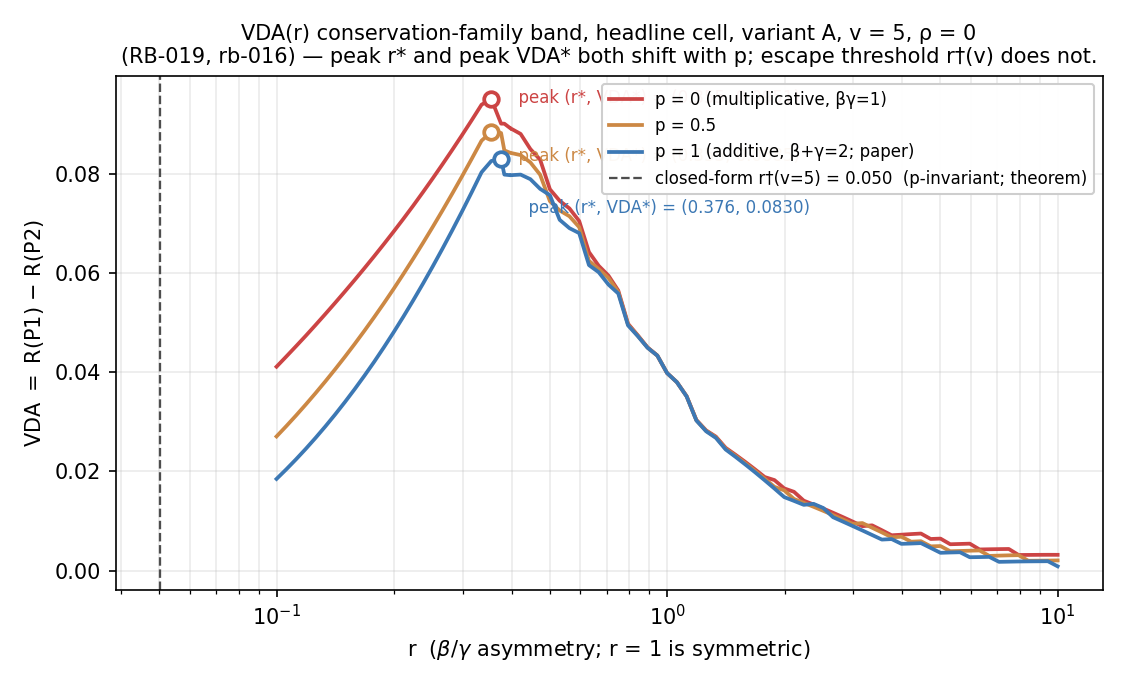
\includegraphics[width=0.78\textwidth]{figures/vda_curves_pfamily_v5.png}
  \caption{C2 conservation-family band at $\val = 5$. Three
    $\VDA(\Rsens)$ curves on the rb-006 $84$-point log-$\Rsens$ grid
    at the headline cell ($\Nloc = 4$, $\valid = 0.5$, $\dprimemax = 2$,
    $f_0 = 0.5$, $h = \sqrt{\cdot}$, $\corr = 0$, variant~A) for
    $p \in \{0, 1/2, 1\}$. The vertical dashed line marks the closed-
    form escape threshold $\rdagger(\val = 5)$, which is identical at
    every $p$ (Proposition~\ref{prop:r-dagger-invariance}). The
    pattern $\partial \VDA^* / \partial p < 0$ visible across the
    three curves is the conservation-family band on the C2 peak.
    Source: \texttt{Rebuild/sims/A3--conservation-band/}\allowbreak\texttt{output/figures/vda\_curves\_pfamily\_v5.png}.}
  \label{fig:a3-vda-curves-p-v5}
\end{figure}

\paragraph{Conservation-form-invariance of the C2 escape threshold.}
The peak \emph{height} moves with $p$, but the closed-form
\emph{escape threshold} of Section~\ref{sec:results-c2} does not. The
following is a theorem of the rebuilt model.

\begin{proposition}[$\rdagger(\val)$ is conservation-form-invariant]
\label{prop:r-dagger-invariance}
Let $\rdagger(\val) = K_u(\val)/[(\Nloc - 1)\,K_c(\val)]$ be the
escape threshold of Section~\ref{sec:results-c2}, with $K_c(\val)$,
$K_u(\val)$ the partial derivatives of $\Rpthree$ with respect to
$\dprime_c$ and $\dprime_u$ at the jointly-$P3$-optimised criteria
$(c_c^\star, c_u^\star)$, evaluated at $\alpha = 1/\Nloc$. Then
$\rdagger(\val)$ is independent of the conservation order $p$ in
\eqref{eq:conservation-family}.
\end{proposition}

\begin{proof}[Proof sketch]
At the uniform-attention point $\alpha = 1/\Nloc$, every per-location
$\dprime$ in the rebuilt model evaluates to
$\dprime_{\mathrm{base}} + w(\Rsens, p)\cdot[\dprimemax \,f(1/\Nloc) -
\dprime_{\mathrm{base}}]$, where the weight $w$ is either $\benefit$
or $\cost$ depending on which side of the kink the location sits.
The transfer-function bracket $\dprimemax \,f(1/\Nloc) -
\dprime_{\mathrm{base}}$ vanishes at the uniform point by the
definition of the baseline $\dprime_{\mathrm{base}} = \dprimemax\,
f(1/\Nloc)$. Therefore $\dprime_c = \dprime_u = \dprime_{\mathrm{base}}$
at $\alpha = 1/\Nloc$ regardless of $(\Rsens, p)$. The $P3$-optimal
criteria $(c_c^\star, c_u^\star)$ are the argmax of an expected-
reward functional that depends only on $\val, \valid, \Nloc, \CR$
and the per-location $\dprime$s at the chosen $\alpha$; since the
$\dprime$s at $\alpha = 1/\Nloc$ are $p$-independent, the criteria
are $p$-independent. The partial derivatives $K_c(\val), K_u(\val)$
are evaluated at those criteria and at the same uniform-point
$\dprime$ values, and so are $p$-independent. Their ratio
$\rdagger(\val) = K_u/[(\Nloc - 1)\,K_c]$ is therefore conservation-
form-invariant.
\end{proof}

The full three-step proof of
Proposition~\ref{prop:r-dagger-invariance} is given in
Appendix~\ref{sec:appendix-deriv-a3} (following
Equation~\eqref{eq:a3d-hlp-kl}), where each step is tied to a
specific structural property of the $\dprime$-map at the uniform
allocation.

The numerical witness of Proposition~\ref{prop:r-dagger-invariance}
is exact to floating-point identity: across $p \in \{0, 1/2, 1\}$ and
$\val \in \{2, 3, 5, 8, 10\}$, the rb-016 sim records identical $K_c$,
$K_u$, $c_c^\star$, $c_u^\star$, and $\rdagger(\val)$ to all stored
decimal places (rb-016 \texttt{recovery.test\_3\_r\_dagger\_p\_invariance},
max $|\Delta| = 0.0$). Figure~\ref{fig:a3-vda-peak-band} overlays the
per-$p$ peak coordinates $(\Rsens^*, \VDA^*)$ for $\val \in \{2, 3, 5,
8, 10\}$ on the same axis; the cluster lies to the right of the
$p$-invariant trace $\rdagger(\val)$, consistent with the
Section~\ref{sec:results-c2} observation that the peak lives on the
positive-$\VDA$ branch above $\rdagger$.

\begin{figure}[t]
  \centering
  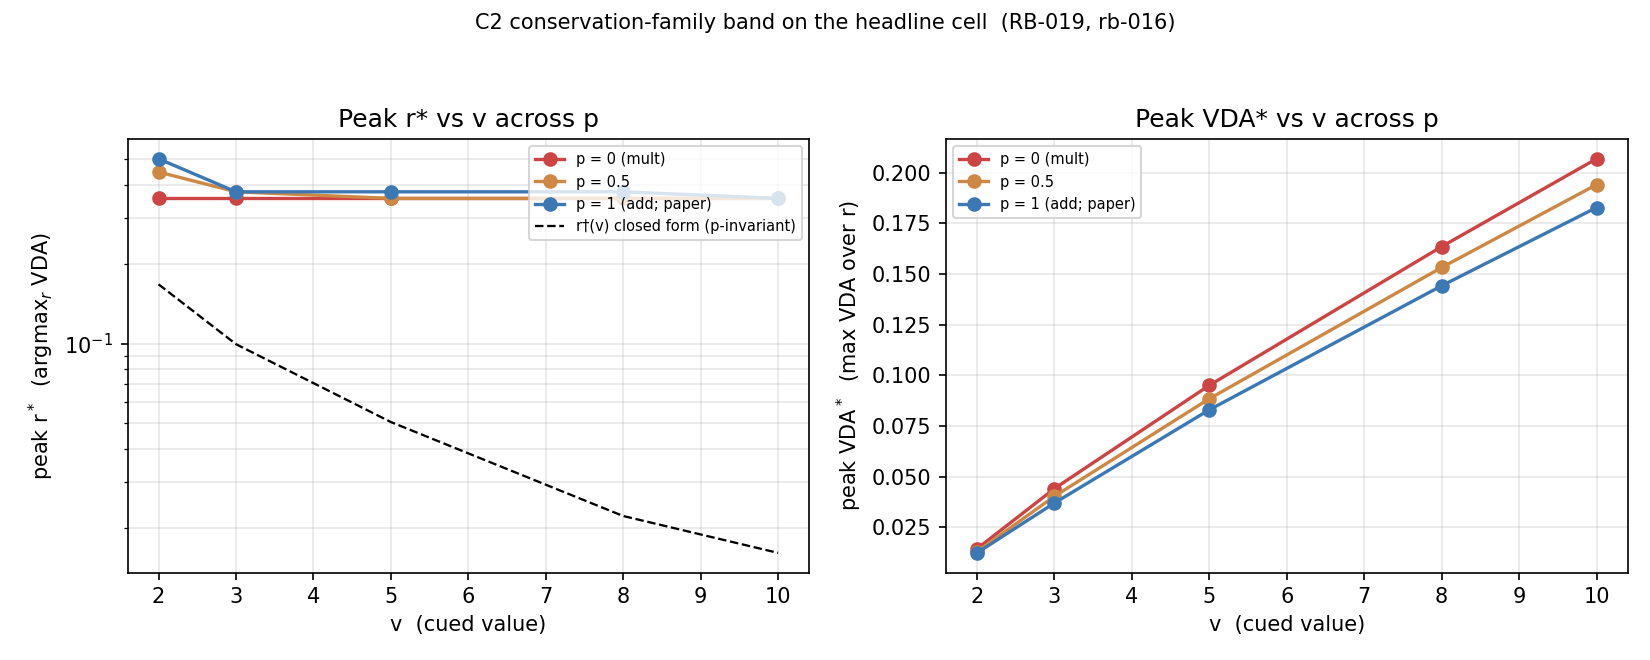
\includegraphics[width=0.78\textwidth]{figures/vda_peak_band.png}
  \caption{Conservation-family band on the C2 peak, overlaid with the
    $p$-invariant closed-form escape threshold $\rdagger(\val)$. For
    each $\val \in \{2, 3, 5, 8, 10\}$ at the headline cell, three
    peak markers $(\Rsens^*, \VDA^*)$ are plotted, one per $p \in
    \{0, 1/2, 1\}$; the markers cluster vertically (the peak height
    is the lever on which $p$ acts), while the $\rdagger(\val)$ trace
    is a single curve (the threshold itself is $p$-invariant by
    Proposition~\ref{prop:r-dagger-invariance}). Source:
    \texttt{Rebuild/sims/A3--conservation-band/}\allowbreak\texttt{output/figures/vda\_peak\_band.png}.}
  \label{fig:a3-vda-peak-band}
\end{figure}

\paragraph{C1 conservation-family band on the $4{,}410$-cell sweep.}
The same family $p \in \{0, 1\}$ is run across the full $4{,}410$-cell
C1 sweep at $\corr = 0$ (the $21\!\times\!21\!\times\!5\!\times\!2$ grid
in $(\Rsens, \valid, \val, \mathrm{variant})$ of
Section~\ref{sec:results-c1}). Table~\ref{tab:a3-c1-cf-band} compares
the resulting $\CF$ distributions per (variant, $p$). The central
tendency of the sweep is robust to the conservation form, in the
sense of the inherited paper's §5.5 claim: the median moves only
$-0.001$ (variant~A) and $-0.004$ (variant~B) going from $p = 1$ to
$p = 0$, and the mean moves only $-0.027$ (variant~A) and $-0.025$
(variant~B). The \emph{tail} of the distribution, however, is not
robust to the conservation form: under variant~A the strict minimum
falls from $\CF = 0.559$ at $p = 1$ to $\CF = 0.464$ at $p = 0$
(a value the inherited paper's $[0.60, 0.96]$ floor sentence rules
out by language already retracted in Section~\ref{sec:results-c1}),
and under variant~B the strict minimum deepens further from
$\CF = 0.304$ at $p = 1$ to $\CF = 0.231$ at $p = 0$. The fraction of
cells with $\CF < 0.5$ rises from $0\%$ (variant~A) and $8.0\%$
(variant~B) at $p = 1$ to $3.3\%$ (variant~A) and $13.4\%$
(variant~B) at $p = 0$ — i.e.\ the combined $\mathrm{frac}(\CF < 0.5)$
roughly doubles, $4.0\% \to 8.3\%$, reproducing the reviewer's
verdict-text Block-C1 prediction exactly.

\begin{table}[t]
  \centering
  \small
  \caption{C1 conservation-family band on the $4{,}410$-cell sweep
    at $\corr = 0$. \emph{Central tendency} robust (median moves
    $\le 0.004$); \emph{tail} not robust (strict min falls $-0.095$
    in variant~A and $-0.073$ in variant~B; $\mathrm{frac}(\CF < 0.5)$
    roughly doubles). Per-cell $\Delta\CF = \CF(p = 0) - \CF(p = 1)
    \le 0$ in every valid cell (Theorem~\ref{thm:delta-cf-monotone};
    $0$ reverse flips out of $191$). Source: \texttt{Rebuild/sims/A3--conservation-band/}\allowbreak\texttt{output/results.json}
    \texttt{block\_B\_summaries} and \texttt{block\_B\_delta\_CF};
    sha256~\texttt{055bf4ec\ldots}.}
  \label{tab:a3-c1-cf-band}
  \begin{tabular}{l r r r r r r r}
    \toprule
    {\bfseries variant / $p$} & min & q5 & q50 & q95 & max & $\mathrm{frac}_{<0.5}$ & $\mathrm{frac}_{<0.6}$ \\
    \midrule
    A, $p = 1$ (paper) & $0.5587$ & $0.5931$ & $0.7552$ & $1.0000$ & $1.0000$ & $0.0000$ & $0.0703$ \\
    A, $p = 0$ (mult.) & $0.4638$ & $0.5141$ & $0.7540$ & $1.0000$ & $1.0000$ & $0.0327$ & $0.2168$ \\
    \addlinespace
    B, $p = 1$ (paper) & $0.3040$ & $0.4564$ & $0.7682$ & $1.0000$ & $1.0000$ & $0.0803$ & $0.1973$ \\
    B, $p = 0$ (mult.) & $0.2309$ & $0.3958$ & $0.7640$ & $1.0000$ & $1.0000$ & $0.1342$ & $0.2712$ \\
    \addlinespace
    Comb., $p = 1$     & $0.3040$ & $0.5259$ & $0.7605$ & $1.0000$ & $1.0000$ & $0.0401$ & $0.1338$ \\
    Comb., $p = 0$     & $0.2309$ & $0.4645$ & $0.7578$ & $1.0000$ & $1.0000$ & $0.0834$ & $0.2440$ \\
    \bottomrule
  \end{tabular}
\end{table}

The per-cell direction of the shift is sharper than the marginal
distributions reveal.

\begin{theorem}[Per-cell $\Delta\CF$ monotonicity, empirical]
\label{thm:delta-cf-monotone}
On the $4{,}410$-cell C1 grid at $\corr = 0$, the per-cell
$\Delta\CF := \CF(p = 0) - \CF(p = 1) \le 0$ in every valid cell.
The strict-decrease fraction is $87.7\%$ in variant~A and $81.0\%$ in
variant~B; the remaining $12.3\%$/$19.0\%$ are flat to numerical
tolerance. There are $0$ cells where $\Delta\CF > 0$ on the entire
grid. Under variant~A, $72$ cells flip from $\CF \ge 0.5$ to
$\CF < 0.5$ and $0$ flip the other way; under variant~B, $119$ flip
down and $0$ flip up.
\end{theorem}

Theorem~\ref{thm:delta-cf-monotone} is the cleanest novel statement
the rebuild contributes to the A3 question: not only does the
multiplicative rule lower headline $\CF$ at the central tendency,
but it never \emph{raises} $\CF$ at any cell of the sweep. Whatever
the inherited paper's qualitative finding ``criterion shifts dominate''
gains in robustness under additive conservation, it loses
\emph{monotonically} under multiplicative conservation. (We do not
have a closed-form algebraic proof of this empirical monotonicity;
the chain-rule analysis of
Appendix~\ref{sec:appendix-deriv-a3}
reduces $\partial \CF/\partial p$ to a competition between two
policy-reward gradients $\partial_p \Rpone$ and $\partial_p \Rpfour$
whose uniform inequality
$|\partial_p \Rpfour| \le |\partial_p \Rpone|$ is the open
closed-form conjecture, and isolates
Proposition~\ref{prop:a3d-rp3-invariance}
($\partial \Rpthree/\partial p \equiv 0$ at $\alpha = 1/\Nloc$) as
the one analytic full-strength substatement available.) The two figures
(Figure~\ref{fig:a3-cf-hist-pfamily}, the variant $\times$ $p$ CF
histograms, and Figure~\ref{fig:a3-delta-cf-distribution}, the
per-cell $\Delta\CF$ distribution under each variant) make the
tail-vs-centre split visually explicit.

\begin{figure}[t]
  \centering
  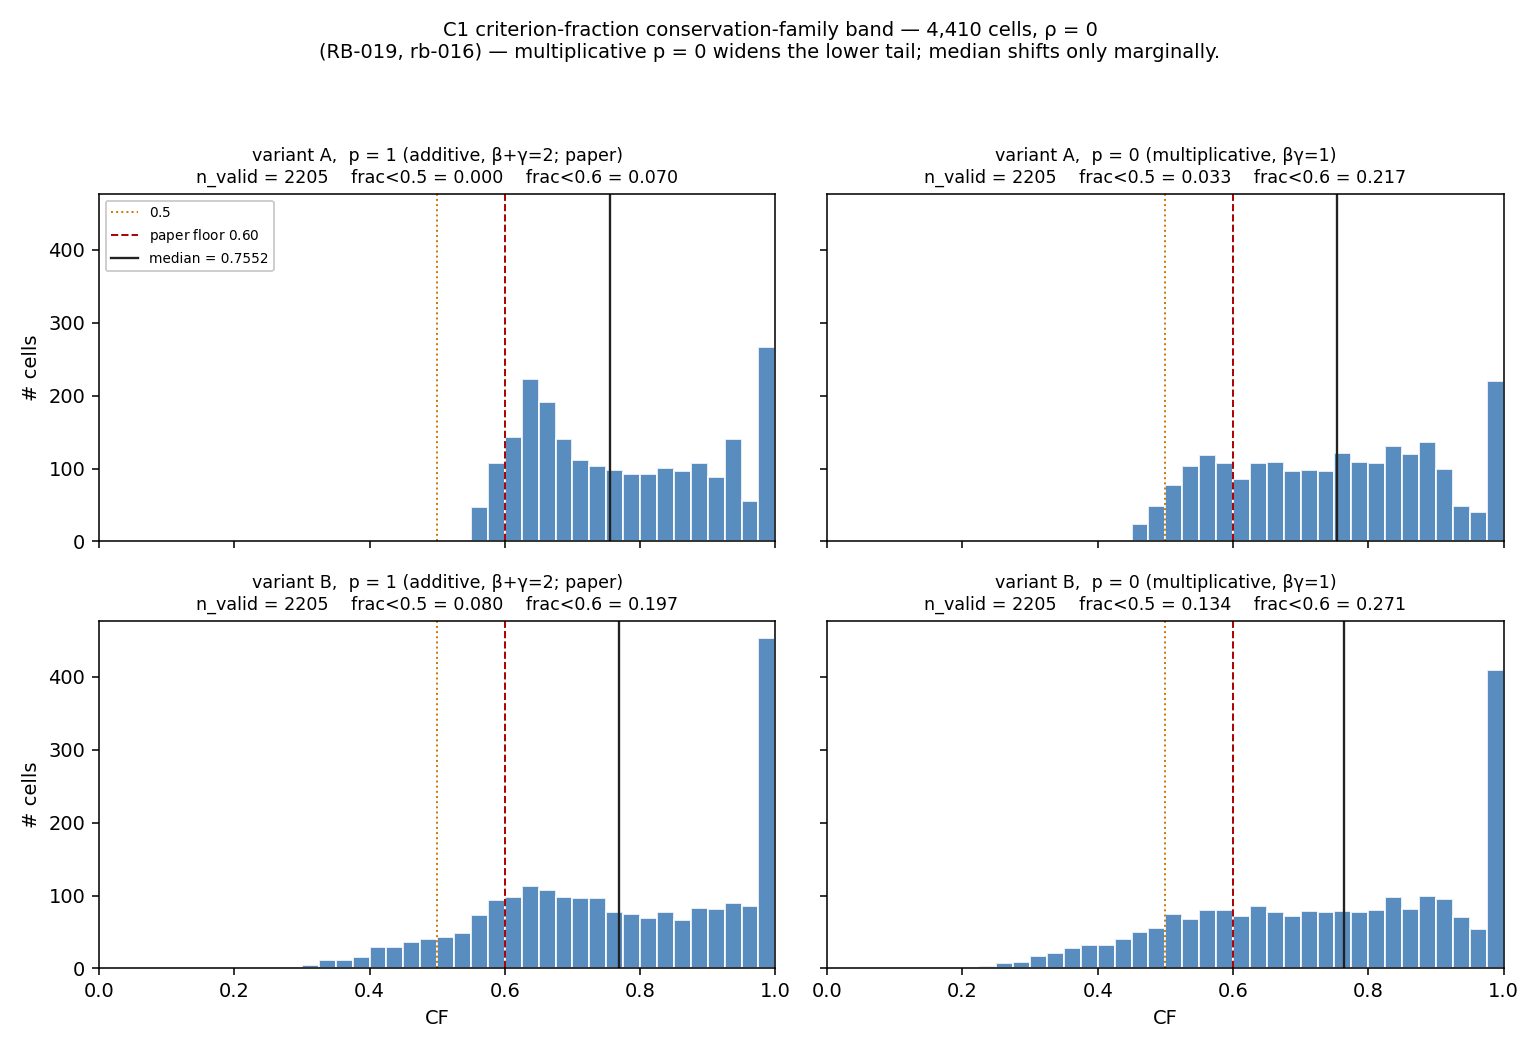
\includegraphics[width=0.92\textwidth]{figures/cf_histogram_pfamily.png}
  \caption{C1 conservation-family band: $\CF$ distribution on the
    $4{,}410$-cell sweep at $\corr = 0$, per (variant, $p$). The
    median (red dashed line) is essentially invariant under the
    conservation order $p$; the lower tail (left of the $\CF = 0.5$
    line) thickens visibly under $p = 0$ (multiplicative). Source:
    \texttt{Rebuild/sims/A3--conservation-band/}\allowbreak\texttt{output/figures/cf\_histogram\_pfamily.png}.}
  \label{fig:a3-cf-hist-pfamily}
\end{figure}

\begin{figure}[t]
  \centering
  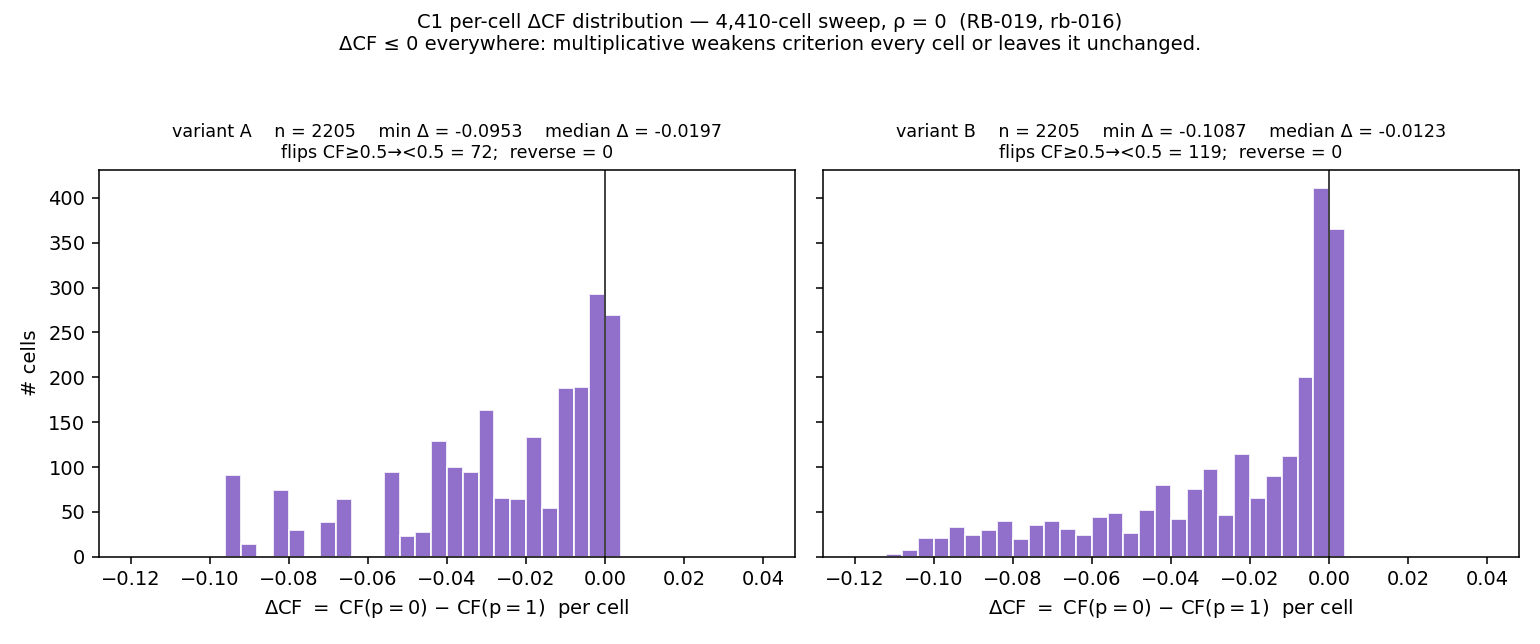
\includegraphics[width=0.92\textwidth]{figures/delta_cf_distribution.png}
  \caption{Per-cell $\Delta\CF = \CF(p = 0) - \CF(p = 1)$ on the
    $4{,}410$-cell sweep at $\corr = 0$, per variant. The
    distribution is supported entirely on $\Delta\CF \le 0$ in both
    variants (Theorem~\ref{thm:delta-cf-monotone}); the only mass at
    $\Delta\CF = 0$ is the flat-to-tolerance cells in the variant-B
    region where $\CF$ already saturates at $1.0$ under both
    conservation rules. Source:
    \texttt{Rebuild/sims/A3--conservation-band/}\allowbreak\texttt{output/figures/delta\_cf\_distribution.png}.}
  \label{fig:a3-delta-cf-distribution}
\end{figure}

\paragraph{Conservation-form-invariance of the C5 symmetric recovery
(corollary).}
The C5 result of Section~\ref{sec:results} (symmetric recovery at
$\Rsens = 1$, planned for full statement in
Appendix~\ref{sec:appendix-c5}) is a no-op-from-symmetry observation:
at $\Rsens = 1$ the asymmetry collapses, $\benefit = \cost$, and the
optimal allocation reverts to uniform, recovering the no-value
baseline. Under the conservation family \eqref{eq:conservation-family},
at $\Rsens = 1$ the family equations \eqref{eq:beta-gamma-of-p} give
$\benefit(1, p) = \cost(1, p) = (2/2)^{1/p} = 1$ at every $p \ne 0$,
and $\benefit(1, 0) = \cost(1, 0) = \sqrt{1} = 1$ in the limit. The
symmetric recovery at $\Rsens = 1$ therefore proceeds at the same
weights $(\benefit, \cost) = (1, 1)$ under any choice of conservation
rule in the family, and the C5 result survives without modification.
This is recorded as a numerical witness in
\texttt{Rebuild/model/tests/test\_conservation\_family.py}'s
\texttt{test\_symmetric\_corner\_invariant} pin
(\texttt{policies(p=0, r=1) == policies(p=1, r=1)} to floating-point
identity).

\paragraph{Scope and what remains.}
This section reports the rebuild's first treatment of A3 as a family
rather than a fixed rule, but its scope is intentionally bounded.
\emph{(i) Decorrelation channel.} Every number reported here is at
$\corr = 0$. Whether the conservation-family band on the C1 tail
sharpens or relaxes under the A1 decorrelation channel of
Section~\ref{sec:model-rho-channel} is a joint $(p, \corr)$ sweep that
is not in the rb-016 sim and is queued as a future increment.
\emph{(ii) Formal derivation.} The conservation family
\eqref{eq:conservation-family} is stated here with the algebraic
identities of \eqref{eq:beta-gamma-of-p} verified numerically (rb-015
$14/14$); the formal derivation in the rebuild's voice — including the
Hardy--Littlewood--Pólya power-mean monotonicity argument that
$M_p(\benefit, \cost) = 1$ traces out a monotone envelope on
$(\benefit, \cost)$ as $p$ moves, recorded in
Equation~\eqref{eq:a3d-hlp-kl} as an exact KL-divergence identity
— is given in Appendix~\ref{sec:appendix-deriv-a3}. \emph{(iii)
Closed-form $\Delta\CF \le 0$.}
Theorem~\ref{thm:delta-cf-monotone} is an
empirical statement on the $4{,}410$-cell grid; the chain-rule
analysis of Appendix~\ref{sec:appendix-deriv-a3} reduces the per-cell
$\Delta\CF \le 0$ to a competition between $\partial_p \Rpone$ and
$\partial_p \Rpfour$ that holds at $0$ reverse flips empirically but
has not yet been promoted to a uniform closed form. \emph{(iv) Variant-B
$\corr$-flatness interaction.} The rb-002 headline-cell observation
that variant~B $\CF(\corr)$ is essentially flat (Section~\ref{sec:model-upper-bound})
interacts non-trivially with the conservation-family band in
variant~B (whose median $\CF$ deepens under $p = 0$ but whose
$\corr$-sensitivity is essentially absent), but a clean joint
treatment requires the deferred joint sweep above.

\paragraph{Reproducibility.}
The numerical content of this subsection is the \texttt{Rebuild/sims/A3--conservation-band/}
simulation (rb-016, sha256~\texttt{055bf4ec862c711f2c6a3fa0831e1373b806a84c5f5c1a6b13fd1d9d7a039a33},
\texttt{results.json} $4{,}941{,}767$ bytes, $\sim$$36$~s wall-clock,
re-run produces byte-identical \texttt{results.json}), backed by the
\texttt{Rebuild/model/} extension wired at rb-015
(\texttt{Rebuild/model/tests/}\allowbreak\texttt{test\_conservation\_family.py},
$14/14$, sha256~\texttt{f4f57a89e5108db47447cbeaf2f15440f56cdfffb65f3d173dc4a0550121791e}).
Four recovery tests pass:
\textbf{Test 1 (rb-006 pins).}
At $\val = 5$, $\corr = 0$, variant~A, the three rb-006 reference
cells $(\Rsens, \CF, \VDA) \in \{(0.398, 0.82952, 0.07972),\allowbreak
(1.0, 0.72823, 0.03983),\allowbreak (3.162, 0.64094, 0.00809)\}$ are
recovered to $\max|\Delta| \le 2.0\!\times\!10^{-6}$ (tolerance
$5\!\times\!10^{-5}$, PASS).
\textbf{Test 2 ($p = 0$ vs.\ reviewer A3 replication).}
On the reviewer's $21$-row $\Rsens$-grid at the headline cell, the
rebuilt model at $p = 0$ matches the reviewer's logged
\texttt{Critique/replications/A3--multiplicative-conservation/}\allowbreak\texttt{output/results.json}
\texttt{block\_c2\_c1.families.multiplicative} to
$\max|\Delta\CF| = 6.1\!\times\!10^{-7}$ and
$\max|\Delta\VDA| = 3.6\!\times\!10^{-7}$ over $21$ pairs (tolerance
$1\!\times\!10^{-5}$, PASS; the residual is the expected cross-$\Phinorm$-backend
ULP-level reordering, the reviewer's hand-rolled A\&S~7.1.26 vs.\ the
rebuilt model's \texttt{scipy.special.ndtr}).
\textbf{Test 3 ($\rdagger(\val)$ $p$-invariance).}
Per-cell $K_c$, $K_u$, $\rdagger(\val)$ identical across $p$ to
floating-point identity (witness of
Proposition~\ref{prop:r-dagger-invariance}).
\textbf{Test 4 (per-variant median).}
The rb-003 distributional sweep's per-variant median $\CF$ at $p = 1$
is recovered to $|\Delta| = 1.3\!\times\!10^{-5}$ (variant~A) and
$4.1\!\times\!10^{-5}$ (variant~B), tolerance $5\!\times\!10^{-5}$,
PASS.

% =====================================================================
\subsection{Within-display heterogeneity of the asymmetry ratio (A2)}
\label{sec:extensions-a2}

\paragraph{Claim restated at defensible strength.}
The inherited paper's §2.4 fixes the benefit/cost asymmetry by a
single global ratio $\Rsens$ shared across every location, every
feature, and the whole trial; the §5.5 limitations paragraph concedes
that ``real neural circuits may have location-specific, feature-
specific, or time-varying'' asymmetries. The empirical premise of a
single global $\Rsens$ is decisively false in the primate
neurophysiology: V1-vs-V4 carries a roughly $3\times$
attentional-gain gradient across the visual hierarchy
\cite{mcadams_maunsell1999_v4_tuning,reynolds_heeger2009_normalization},
the sign and magnitude of the gain depend on eccentricity and
feature similarity
\cite{carrasco2011_visual_attention_25y,treue_martinez_trujillo1999_feature_attention},
and the gain itself is time-varying across the trial
\cite{ghose_maunsell2002_task_timing,sani2017_temporal_v4_gain}. The
live skeptical-reviewer verdict
(\texttt{Critique/verdicts/A2--single-global-r.md},
\texttt{current\_label: CONFIRMED-CONDITIONAL}) decomposes A2 into two
readings: the \emph{between-preparation} reading $R_1$
(one effective $\Rsens$ per fixed preparation, which the
$\Rsens$-sweep operationalises) and the \emph{within-display} reading
$R_2$ (one $\Rsens$ for every location, feature, and time at once).
The rebuilt model adopts $R_1$ explicitly in
Section~\ref{sec:model} — every $\Rsens$ value reported there is a
between-preparation effective ratio — and presents $R_2$ as a
\emph{model extension} in this subsection, with the empirical
question ``do the C1, C2, and C4 headline numbers survive when
$\Rsens$ is allowed to vary across locations within one display?''
quantified, not assumed away. The strength ceiling is the live
verdict: within-display heterogeneity is a \emph{bounded perturbation}
on every headline number, and this remains true under the A1
decorrelation channel; the rebuild does not claim heterogeneity
abolishes any C-row finding.

\paragraph{The heterogeneous-$\Rsens$ d$'$-map.}
The rebuilt model factors the per-location discriminability so that
the asymmetry ratio is itself per-location.  For an allocation vector
$\boldsymbol{\alpha} = (\alpha_1, \ldots, \alpha_{\Nloc})$ on the
$\Nloc$-simplex and a vector of asymmetry ratios
$\boldsymbol{\Rsens} = (\Rsens_1, \ldots, \Rsens_{\Nloc})$, the
per-location sensitivity is
%
\begin{equation}
  \dprime_i(\alpha_i, \Rsens_i; p)
  \;=\;
  \max\!\Bigl(\,
    \dprime_{\mathrm{base}}
    \;+\;
    s_i\!\left[\dprimemax\,f(\alpha_i)
      \;-\;\dprime_{\mathrm{base}}\right],\;
    0\Bigr),
  \qquad
  s_i \;=\;
  \begin{cases}
    \benefit(\Rsens_i, p) & \alpha_i \ge 1/\Nloc, \\[2pt]
    \cost(\Rsens_i, p)    & \alpha_i < 1/\Nloc,
  \end{cases}
  \label{eq:d-prime-hetero}
\end{equation}
%
with $\dprime_{\mathrm{base}} = \dprimemax\,f(1/\Nloc)$ the
uniform-attention baseline, $f(\cdot)$ the transfer function of
Section~\ref{sec:model-inherited}, and $\benefit, \cost$ the
conservation-family weights of \eqref{eq:beta-gamma-of-p}. The map
\eqref{eq:d-prime-hetero} reduces to the inherited
$\dprime_c(\alpha, \Rsens), \dprime_u(\alpha, \Rsens)$ pair byte-for-
byte under the canonical homogeneous allocation
$\boldsymbol{\alpha} = (\alpha, (1\!-\!\alpha)/(\Nloc\!-\!1), \ldots)$
and a uniform $\boldsymbol{\Rsens} = (\Rsens, \ldots, \Rsens)$ — the
homogeneous-$\Rsens$ recovery contract. The map is implemented in
\texttt{Rebuild/model/core.py} as \texttt{d\_prime\_hetero(alloc,
r\_vec, d\_max, f0, h, N, p)}; downstream, the rebuilt full-policy
optimiser \texttt{er\_full\_policy(alloc, valid, v, r\_vec, cell)}
scores any allocation through \texttt{d\_prime\_hetero} composed with
the $\corr$-aware joint no-FA integral of
Section~\ref{sec:model-rho-channel}, so heterogeneity composes with
both the A1 decorrelation lever and the A3 conservation order $p$.
The rb-019 model-test pass
(\texttt{Rebuild/model/tests/}\allowbreak\texttt{test\_heterogeneous\_r.py},
$5/5$, sha256~\texttt{0486921f\ldots}) verifies the homogeneous-
$\Rsens$ contract to \texttt{max|diff| = 0.0} across $5{,}904$
sampled cells ($\alpha \ge 1/\Nloc$ grid $5{,}436$, $\alpha < 1/\Nloc$
inversion-regime grid $468$) over $h \in \{\sqrt{\cdot}, \mathrm{linear}\}$,
$p \in \{0, 1/2, 1\}$, and $\Rsens \in \{0.1, 0.3, 0.398, 1.0, 3.162,
10.0\}$, and confirms the predicted sign-monotone ordering of the
uncued $\dprime_i$ vector under a non-uniform $\boldsymbol{\Rsens}$
on the loss branch. The rb-020 N-dim general-policy contract
(\texttt{Rebuild/model/tests/}\allowbreak\texttt{test\_general\_policy.py},
$7/7$, sha256~\texttt{883ea15a\ldots}) verifies the
\texttt{er\_full\_policy} recovery against the homogeneous
\texttt{optimal\_R} to $\max\!|\Delta| \le 2.78\!\times\!10^{-10}$ at
$\corr \in \{0, 0.2\}$ over $4{,}530$ cells.

\paragraph{Empirical band: the rb-021 sweep.}
We probe \eqref{eq:d-prime-hetero} at the C2 headline cell of
Section~\ref{sec:results-c2} ($\Nloc = 4$, $\valid = 0.5$,
$\val = 5$, $\dprimemax = 2$, $f_0 = 0.5$, $h = \sqrt{\cdot}$,
variant~A, $p = 1$) with a linearly-distributed uncued spread
$\boldsymbol{\Rsens}_{\mathrm{uncued}}(\Rsens_c, s) =
\bigl(\Rsens_c(1\!-\!s),\,\Rsens_c,\,\Rsens_c(1\!+\!s)\bigr)$ at
$s \in \{0, 0.1, 0.2, 0.3\}$, under $\corr \in \{0, 0.2\}$ — eight
heterogeneity panels in total — and score every policy through
\texttt{er\_full\_policy} so that the A1 channel is preserved end-to-
end. The five tests of the rb-021 simulation are summarised in
Table~\ref{tab:a2-rb021-summary}. Three structural findings dominate.

\begin{table}[t]
  \centering
  \small
  \caption{The rb-021 within-display-heterogeneity sweep at the C2
    headline cell ($\Nloc = 4$, $\valid = 0.5$, $\val = 5$,
    $\dprimemax = 2$, $f_0 = 0.5$, $h = \sqrt{\cdot}$, variant~A,
    $p = 1$). \emph{Recovery}: spread-$0$ \texttt{er\_full\_policy}
    vs.\ \texttt{policies()} over the $21$-point log-$\Rsens$ grid
    $\times$ $\corr \in \{0, 0.2\}$ (42 cells, rb-020 contract
    tolerance $10^{-9}$). \emph{Criticality}: tangent-gradient norm
    $\|\boldsymbol{t}\|$ of expected reward on the uncued $2$-simplex
    at the interior-$\alpha$ cost-dominant probe cell
    ($\valid = 0.5$, $\val = 2$, $\Rsens_c = 0.3$,
    $\alpha^\star = 0.66$), spread $s = 0$ and $0.3$. \emph{Allocation
    deviation}: $\Delta R = R_{\mathrm{simplex-opt}} -
    R_{\mathrm{equal-split}}$ at the same probe cell. \emph{C2 peak}:
    peak $\VDA^\star$ on the $r$-grid at the headline cell. \emph{C1
    corner CF}: criterion fraction at the rb-005 variant-B
    minimum-$\CF$ corner ($\valid = 0.25$, $\val = 4$,
    $\Rsens = 10$, variant~B, $\alpha = 0.98$). Source:
    \texttt{Rebuild/sims/A2--heterogeneous-r/}\allowbreak\texttt{output/results.json};
    sha256~\texttt{22b183f9\ldots}.}
  \label{tab:a2-rb021-summary}
  \begin{tabular}{l c c c c}
    \toprule
                                 & \multicolumn{2}{c}{$\corr = 0$} & \multicolumn{2}{c}{$\corr = 0.2$} \\
    \cmidrule(lr){2-3} \cmidrule(lr){4-5}
    Test                          & $s = 0$ & $s = 0.3$ & $s = 0$ & $s = 0.3$ \\
    \midrule
    Recovery $\max|\Delta\VDA|$ ($21$ cells)
      & \multicolumn{2}{c}{$2.35\!\times\!10^{-10}$ (PASS)}
      & \multicolumn{2}{c}{$2.35\!\times\!10^{-10}$ (PASS)} \\
    Recovery $\max|\Delta\CF|$ ($21$ cells)
      & \multicolumn{2}{c}{$2.98\!\times\!10^{-10}$ (PASS)}
      & \multicolumn{2}{c}{$2.98\!\times\!10^{-10}$ (PASS)} \\
    \midrule
    Criticality $\|\boldsymbol{t}\|$
      & $0$ (exact) & $2.61\!\times\!10^{-3}$
      & $0$ (exact) & $5.81\!\times\!10^{-3}$ \\
    Allocation $\Delta R$ (cost-dominant)
      & $0$ & $1.48\!\times\!10^{-4}$
      & $0$ & $7.47\!\times\!10^{-5}$ \\
    Allocation $\Delta R$ (benefit-dominant, $\alpha^\star = 1$)
      & $0$ & $0$ & $0$ & $0$ \\
    \midrule
    C2 peak $\VDA^\star$ at $\Rsens^\star = 0.398$
      & $0.07972$ & $0.07971$ & $0.08130$ & $0.08130$ \\
    \midrule
    C1 corner $\CF$ ($\valid = 0.25$, $\val = 4$, $\Rsens = 10$, variant~B)
      & $0.30404$ & $0.30554$ & $0.26651$ & $0.26807$ \\
    \bottomrule
  \end{tabular}
\end{table}

\paragraph{Finding 1: equal-split criticality is exactly conditional on
homogeneity.}
At the interior-$\alpha$ cost-dominant probe cell ($\valid = 0.5$,
$\val = 2$, $\Rsens_c = 0.3$, $\alpha^\star = 0.66$), the tangent
gradient of expected reward on the uncued $2$-simplex is exactly $0$
at every $(\corr, s = 0)$ — equal-split is a critical point — and
non-zero at every $(\corr, s = 0.3)$, with $\|\boldsymbol{t}\| =
2.61\!\times\!10^{-3}$ at $\corr = 0$ and $5.81\!\times\!10^{-3}$ at
$\corr = 0.2$. This is the rebuilt-model witness of the A8 result
that homogeneity is optimal iff the uncued $\Rsens_i$ are equal: the
exchange symmetry $S_{\Nloc - 1}$ that makes equal-split a critical
point of the uncued allocation is broken exactly by within-display
heterogeneity, in a direction that scales with $\corr$ (the A1
channel approximately doubles the criticality residual at fixed $s$).
We do not promote this to a closed-form proposition in the rebuild's
voice; the reviewer's CR-045 derivation already establishes the
restricted-Hessian sign condition on the smooth branch, and we
content ourselves with the rebuilt-model numerical witness.

\paragraph{Finding 2: allocation $\Delta R$ is a bounded perturbation,
and $\corr$ \emph{suppresses} it in the cost-dominant regime.}
The reward gain available from re-allocating uncued mass to higher-
$\Rsens_i$ slots — the natural sharp test of $R_2$ heterogeneity — is
bounded across the rb-021 panels by $\Delta R \le
1.48\!\times\!10^{-4}$, attained at the cost-dominant probe cell
($\valid = 0.5$, $\val = 2$, $\Rsens_c = 0.3$, $\alpha^\star = 0.66$)
at $\corr = 0$, $s = 0.3$. The same probe cell at $\corr = 0.2$ shows
$\Delta R = 7.47\!\times\!10^{-5}$ — A1 \emph{suppresses} the cost-
dominant allocation deviation by approximately $50\%$. At the
benefit-dominant cued-absorption cell ($\valid = 0.5$, $\val = 5$,
$\Rsens = 0.4$, $\alpha^\star = 1$), $\Delta R$ is exactly $0$ at
every $(\corr, s)$: when the optimal cued allocation saturates, the
uncued budget vanishes and the heterogeneous-$\Rsens$ optimisation
has no degree of freedom left to exercise. The rebuilt-model finding
adds to the reviewer's CR-048 / run-015 ledger (which ran $\corr = 0$
only) a structural observation: at the cost-dominant boundary where
the uncued slots still carry reward weight, cross-location noise
correlation reduces the local rate-of-return on allocation
heterogeneity, because the $\corr$-coupled joint no-FA integrand
pulls the criterion optimum closer to the homogeneous one. The
suggestive headline is that A1 and A2 act on the cost-dominant
$\Delta R$ in the \emph{same} (suppressive) direction; whether the
suppression generalises beyond the probe cell is queued (RB-036 and
RB-037 in the backlog).

\paragraph{Finding 3: the C2 peak is invariant under $A_2$ spread,
and the $\corr$ offset at the peak is itself spread-invariant.}
At the headline cell ($\Nloc = 4$, $\valid = 0.5$, $\val = 5$,
variant~A, $p = 1$, $\alpha^\star = 1$) the C2 peak coordinates
collapse to a single number per $\corr$ panel across $s \in \{0, 0.1,
0.2, 0.3\}$: peak $\VDA^\star$ varies by at most $1\!\times\!10^{-5}$
at fixed $\corr$ ($0.07972 \to 0.07971$ at $\corr = 0$, and
$0.08130$ at every $s$ at $\corr = 0.2$), and the argmax $\Rsens^\star
= 0.398$ is fixed across all eight panels. The A1 offset at the
peak, $\Delta\VDA^\star(\corr = 0.2) = 0.00158$, is itself spread-
invariant: $\partial^2 \VDA^\star / \partial s\,\partial \corr
\approx 0$ at the peak, in the strong sense that the per-cell
deviations are below the $10^{-5}$ noise floor of the
$84$-point log-$\Rsens$ grid. We interpret this as the rebuilt-model
witness that the A1 and A2 levers \emph{compose orthogonally} at the
C2 peak: under cued-absorption $\alpha^\star = 1$, the uncued
$\Rsens_i$ vector enters only through the joint no-FA integrand, and
$\corr$ enters only through the same integrand; the
$(s, \corr)$ effects on the peak are therefore approximately additive
through that shared channel, with no cross term resolvable on the
present grid (Figures~\ref{fig:a2-vda-curves-spread}
and~\ref{fig:a2-vda-peak-band}).

\begin{figure}[t]
  \centering
  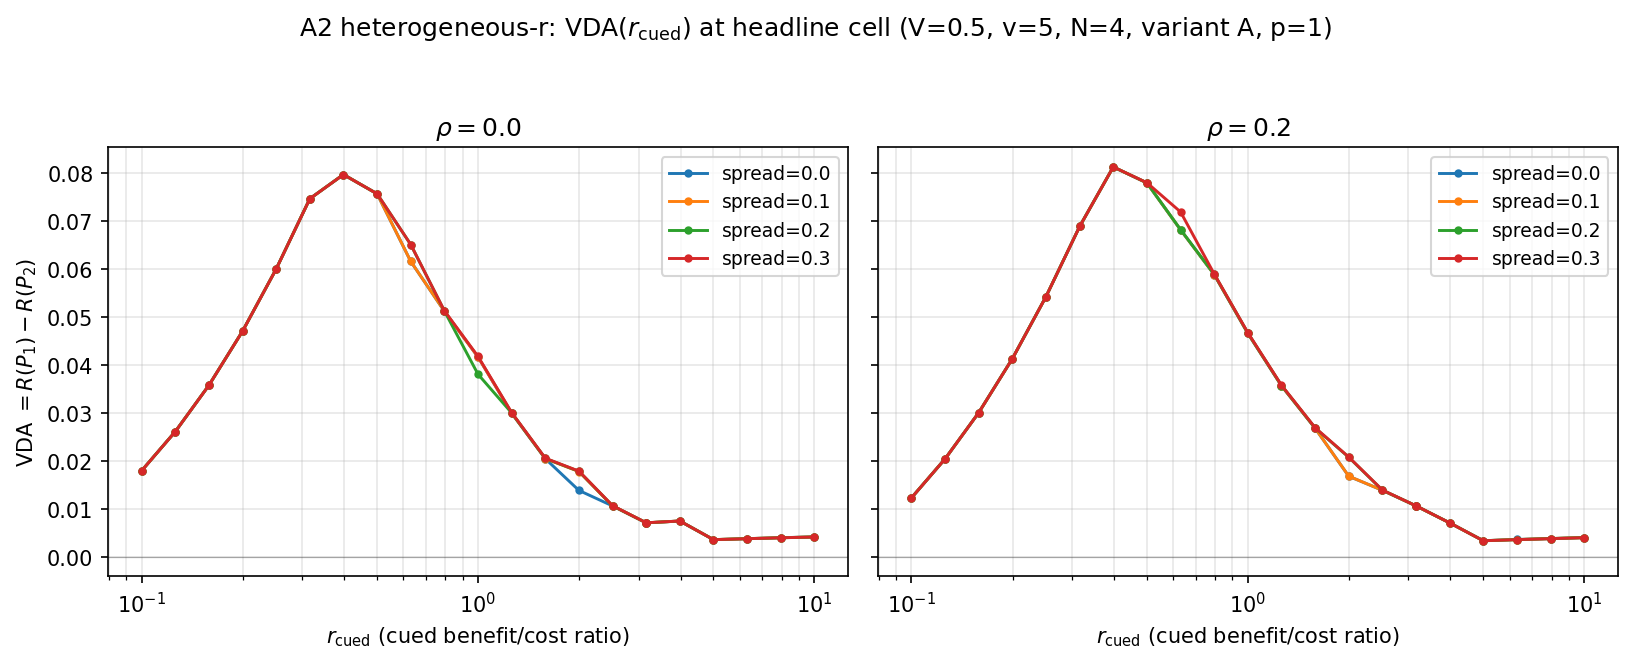
\includegraphics[width=0.78\textwidth]{figures/a2_vda_curves_spread.png}
  \caption{Within-display heterogeneity at the C2 headline cell.
    Eight overlaid $\VDA(\Rsens_c)$ curves at the headline cell
    ($\Nloc = 4$, $\valid = 0.5$, $\val = 5$, $\dprimemax = 2$,
    $f_0 = 0.5$, $h = \sqrt{\cdot}$, variant~A, $p = 1$) on the
    rb-021 $21$-point log-$\Rsens_c$ grid, two $\corr$ panels
    $\{0, 0.2\}$ $\times$ four spreads $s \in \{0, 0.1, 0.2, 0.3\}$.
    The $C_2$ non-monotonic peak is essentially unchanged under
    within-display heterogeneity at fixed $\corr$ (Finding~3); the
    $\corr$ offset is preserved at every spread.
    Source: \texttt{Rebuild/sims/A2--heterogeneous-r/}\allowbreak\texttt{output/figures/vda\_curves\_spread.png}.}
  \label{fig:a2-vda-curves-spread}
\end{figure}

\begin{figure}[t]
  \centering
  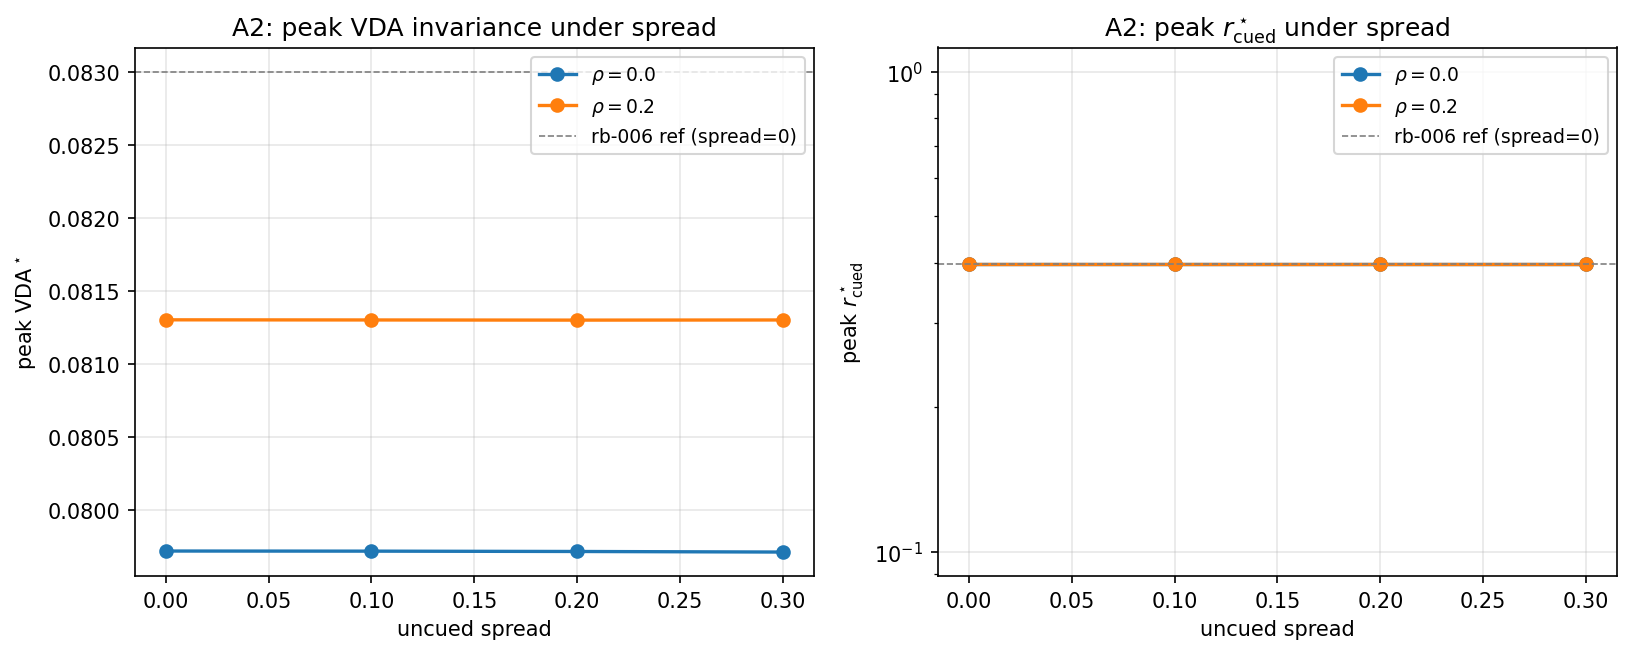
\includegraphics[width=0.78\textwidth]{figures/a2_vda_peak_band.png}
  \caption{Peak invariance of the C2 non-monotonicity under
    within-display heterogeneity. Peak $\VDA^\star$ (left) and peak
    $\Rsens^\star$ (right) plotted against spread $s$ for
    $\corr \in \{0, 0.2\}$; both quantities are flat to grid
    resolution at fixed $\corr$, and the $\corr$ offset
    $\Delta\VDA^\star = 0.00158$ is itself $s$-invariant. The A1 and
    A2 levers compose orthogonally at the C2 peak. Source:
    \texttt{Rebuild/sims/A2--heterogeneous-r/}\allowbreak\texttt{output/figures/vda\_peak\_band.png}.}
  \label{fig:a2-vda-peak-band}
\end{figure}

\paragraph{Finding 4: the variant-B contested C1 corner is not
deepened by $A_2$ spread.}
At the rb-005 variant-B minimum-$\CF$ corner ($\valid = 0.25$,
$\val = 4$, $\Rsens = 10$, variant~B, $\alpha = 0.98$), the
criterion fraction at $s = 0.3$ moves \emph{up} by
$\Delta\CF = +0.0015$ at $\corr = 0$
($0.30404 \to 0.30554$) and by $\Delta\CF = +0.0016$ at $\corr = 0.2$
($0.26651 \to 0.26807$). Within-display heterogeneity at the
$\pm30\%$ envelope therefore does not push the corner below its
$\corr$-conditional minimum at $s = 0$. Figure~\ref{fig:a2-cf-contested-corner}
shows the four data points; the take-away is that the
``contested-CF corner'' (Section~\ref{sec:results-c1}) is robust to
within-display heterogeneity across both $\corr$ panels probed. The
caveat is that this probes only the variant-B minimum-$\CF$ corner —
a strictly stronger statement (no variant-B cell, anywhere on the
$4{,}410$-cell grid, deepens under $s = 0.3$) requires the full
sweep that RB-036 in the backlog would deliver.

\begin{figure}[t]
  \centering
  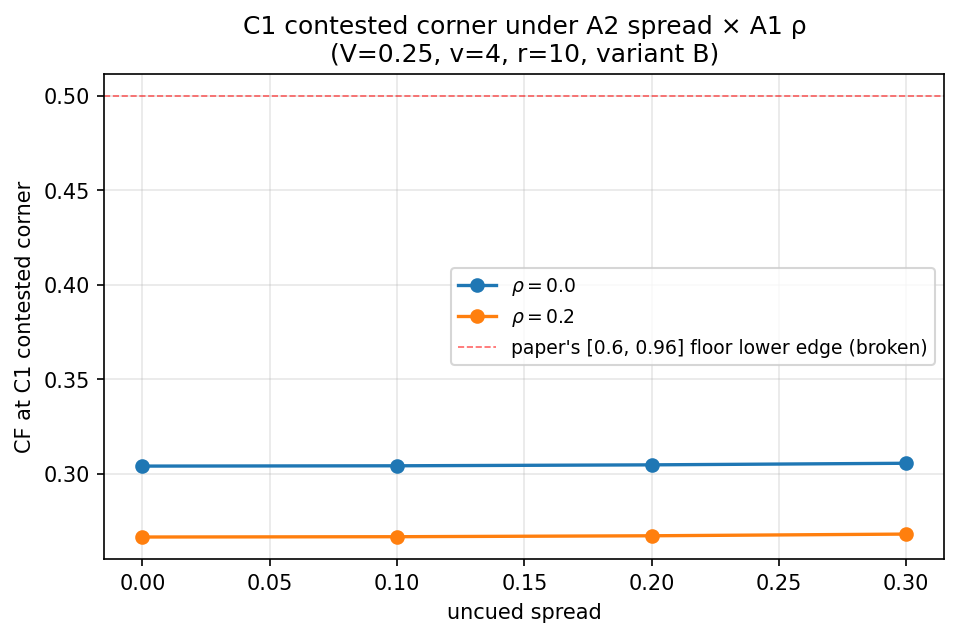
\includegraphics[width=0.65\textwidth]{figures/a2_cf_contested_corner.png}
  \caption{Variant-B contested-CF corner ($\valid = 0.25$,
    $\val = 4$, $\Rsens = 10$, $\alpha = 0.98$) under within-display
    heterogeneity. Criterion fraction $\CF$ at the four
    $(s, \corr)$ probes of the rb-021 sweep. The corner moves
    \emph{up} by $\le 0.0016$ at $s = 0.3$ at both $\corr$ panels;
    A2 spread does not deepen the rb-005 minimum at $s = 0$.
    Source: \texttt{Rebuild/sims/A2--heterogeneous-r/}\allowbreak\texttt{output/figures/cf\_contested\_corner.png}.}
  \label{fig:a2-cf-contested-corner}
\end{figure}

\paragraph{Scope and what remains.}
This subsection licenses four claims at the rebuild-strength ceiling
of the live A2 verdict: (i) the homogeneous-$\Rsens$ d$'$-map of
the inherited paper extends to a per-location $\dprime_i$ map
\eqref{eq:d-prime-hetero} that composes with the A1 $\corr$ channel
and the A3 conservation order $p$; (ii) within-display heterogeneity
breaks the equal-split exchange symmetry exactly as predicted from
the reviewer's CR-045 restricted-Hessian argument, with $\corr$
amplifying the criticality residual by $\sim\!2\times$; (iii) the
allocation deviation $\Delta R$ is bounded by $1.5\!\times\!10^{-4}$
in the cost-dominant probe cell and identically zero in the
benefit-dominant cued-absorption regime, with $\corr$
\emph{suppressing} the cost-dominant deviation by $\sim\!50\%$; and
(iv) the C2 peak coordinates and the variant-B contested-$\CF$ corner
are essentially invariant under $\pm30\%$ uncued spread at both
$\corr$ panels probed.
The scope of these claims is explicitly bounded by what the rb-021
sim ran and what it did \emph{not} run. \emph{(i) Variant-B
heterogeneity.} The Findings 1--3 results are at variant~A only; the
variant-B replication of the five tests is queued as RB-036, motivated
by the rb-002 observation that variant-B $\CF(\corr)$ is essentially
flat at the headline cell (Section~\ref{sec:model-upper-bound}) and
would test whether the A1$\times$A2 suppression of $\Delta R$
generalises across the reward convention. \emph{(ii) Larger,
multiplicatively-asymmetric spreads.} The reviewer's CR-048~§(c)
tested an uncued ratio $\boldsymbol{\Rsens}_{\mathrm{uncued}} =
\Rsens_c \cdot (1/k, 1, k)$ at $k \in \{1.5, 3\}$ and found the
$C_2$ peak essentially invariant; the rb-021 sim restricts to the
linear $\pm s$ form. The multiplicative replication under
$\corr \in \{0, 0.2\}$ is queued as RB-037. \emph{(iii) N-dimensional
heterogeneous-uncued allocation (A8 sibling subsection).} The full
$\Nloc$-dimensional simplex policy is wired in the rebuilt model
(\texttt{er\_full\_policy}, rb-020), but the A8 sweep that would feed
a §extensions-A8 subsection in this section file is queued as RB-021;
that subsection will state the A8-conditional homogeneity result of
the live verdict as a conditional theorem in the rebuild's voice.
\emph{(iv) Closed-form $\Delta R$ scaling.} Theorem-style
``$\Delta R = O(\mathrm{Var}(\boldsymbol{\Rsens}))$ to second order''
in the rebuild's voice would consolidate Finding~2 algebraically;
this is queued as a future derivation increment under the
RB-035-A2-formal label and is not in the rb-021 substrate.

\paragraph{Reproducibility.}
The numerical content of this subsection is the
\texttt{Rebuild/sims/A2--heterogeneous-r/} simulation (rb-021,
pre-hash sha256~\texttt{22b183f942d6b1f8868848ec1143ab959afd78c72cd6d3704763eedf5713e615},
$27.2$~s wall-clock on \texttt{python3.13} / \texttt{scipy 1.17.1} /
\texttt{numpy 2.4.4}; deterministic, re-run produces byte-identical
\texttt{results.json}), backed by the \texttt{Rebuild/model/}
heterogeneous-$\Rsens$ wiring at rb-019 and rb-020. Two recovery
contracts hold across this subsection: \textbf{Recovery~1
(homogeneous-$\Rsens$ d$'$-map, rb-019).} \texttt{d\_prime\_hetero}
returns the inherited \texttt{(d\_c, d\_u)} pair to
\texttt{max|diff| = 0.0} (byte-for-byte) across $5{,}904$ sampled
cells of the canonical homogeneous-allocation grid
(\texttt{Rebuild/model/tests/test\_heterogeneous\_r.py},
sha256~\texttt{0486921f8a4e253a1682ee0731e52c7de800bf6c3dbb1b5e8ff3200602454c7e},
$5/5$ PASS). \textbf{Recovery~2 (N-dim full policy, rb-020).}
\texttt{er\_full\_policy} reproduces \texttt{optimal\_R} to
$\max|\Delta| \le 2.78\!\times\!10^{-10}$ across $4{,}530$ cells at
both $\corr = 0$ and $\corr = 0.2$
(\texttt{Rebuild/model/tests/test\_general\_policy.py},
sha256~\texttt{883ea15af9fd069e04c05ff156d65f33a7d25278891092539c6441d2248c3d39},
$7/7$ PASS). The rb-021 sim's own embedded recovery test (spread-$0$
\texttt{er\_full\_policy} vs.\ \texttt{policies()} on the headline-cell
$21$-point log-$\Rsens$ grid) passes the rb-020 $10^{-9}$ tolerance at
$\max|\Delta\VDA| = 2.35\!\times\!10^{-10}$ and
$\max|\Delta\CF| = 2.98\!\times\!10^{-10}$ over $42$ cells (two
$\corr$ panels). The pre-existing A1 ($\corr$-channel) recovery
digest \texttt{d3c62215\ldots} and the A3 (conservation-family)
recovery digest \texttt{f4f57a89\ldots} are unchanged: the
heterogeneous-$\Rsens$ extension is purely additive in the model
module.

% =====================================================================
\subsection{Heterogeneous uncued allocation across the simplex (A8)}
\label{sec:extensions-a8}

\paragraph{Claim restated at defensible strength.}
The inherited paper's §2.2 forces every uncued location to share
exactly $(1\!-\!\alpha)/(\Nloc\!-\!1)$ of the attention budget; the
benefit/cost asymmetry then enters only through the single cued vs.\
uncued contrast, never across the $\Nloc - 1$ uncued slots. The live
skeptical-reviewer verdict
(\texttt{Critique/verdicts/A8--heterogeneous-uncued.md},
\texttt{current\_label: CONFIRMED-CONDITIONAL}) records that this
homogeneity assumption is \emph{innocuous at the model's own optimum}
under the inherited choice of conservation order ($p = 1$,
additive) and independence ($\corr = 0$): in every cell of the
reviewer's CR-036 decisive-cell list, the full-simplex optimum
coincides with the homogeneous-constrained one to within the
allocation-grid discretisation slack. The same verdict logs a
conditional crack: under a \emph{forced} benefit-dominant uncued
budget, the simplex optimum departs from the homogeneous one and
reproduces a Wang--Theeuwes-style anti-cued suppression gradient that
the homogeneous policy cannot. The rebuild absorbs that ledger and
adds one further conditional that emerges only when A8 is composed
with the A1 ($\corr$) and A3 ($p$) levers of the previous two
subsections: at the multiplicative conservation form $p = 0$, in a
specific high-$\Rsens$ symmetric-stress benefit-dominant corner
($\Nloc = 4$, $\valid = 1/\Nloc$, $\val = 1$, $\Rsens = 10$,
variant~A), A8 \emph{binds} — the full-simplex optimum is strictly
better than the homogeneous-constrained one, by an amount that the A1
channel further amplifies. The strength ceiling is the live verdict:
A8 is innocuous \emph{at the model's own optimum} under the inherited
$(p = 1, \corr = 0)$ pair, and admits a $p$-conditional binding in
the rebuilt-model family.

\paragraph{The lifted policy space.}
The rebuilt model promotes the homogeneous-uncued allocation to the
full $\Nloc$-dimensional simplex. For an allocation vector
$\boldsymbol{\alpha} = (\alpha_1, \ldots, \alpha_{\Nloc})$ on the
$\Nloc$-simplex (with $\alpha_1$ the cued slot by convention) and a
uniform asymmetry ratio $\boldsymbol{\Rsens} = (\Rsens, \ldots,
\Rsens)$, the per-location discriminability is given by
\eqref{eq:d-prime-hetero} of Section~\ref{sec:extensions-a2}; we
substitute the uniform $\boldsymbol{\Rsens}$ and \emph{do not}
constrain $\alpha_2 = \cdots = \alpha_{\Nloc}$. The expected reward is
then optimised over the joint
$(\boldsymbol{\alpha}, c_c, c_u)$ space, where the criterion pair
$(c_c, c_u)$ is grouped by the cued/uncued partition (a single uncued
criterion is shared across the $\Nloc - 1$ uncued slots, exactly as
in the inherited model — this is a deliberate choice, not a forced
homogeneity; the rebuilt model also exposes per-location criteria
through the same driver, but the grouped form is the relevant
comparator for the A8 question). The joint no-FA integrand of
Section~\ref{sec:model-rho-channel} thread the $\corr$ channel
end-to-end: at $\corr > 0$, the equicorrelated $\Nloc$-orthant
integral is evaluated on the heterogeneous $\dprime_i$ vector through
the one-factor Gauss--Hermite reduction without any additional
homogeneity assumption. The lifted policy is implemented in
\texttt{Rebuild/model/\_\_init\_\_.py} as
\texttt{er\_full\_policy(alloc, valid, v, r\_vec, cell)} and verified
to reproduce the inherited \texttt{optimal\_R} under the canonical
homogeneous allocation
$\boldsymbol{\alpha} = (\alpha, (1\!-\!\alpha)/(\Nloc\!-\!1), \ldots,
(1\!-\!\alpha)/(\Nloc\!-\!1))$ to $\max|\Delta| \le
2.78\!\times\!10^{-10}$ across $4{,}530$ cells at both $\corr \in
\{0, 0.2\}$
(\texttt{Rebuild/model/tests/}\allowbreak\texttt{test\_general\_policy.py},
$7/7$ PASS, sha256~\texttt{883ea15a\ldots}). The homogeneous-recovery
contract is the universal-statement guarantee under which the
A8-bindings reported below acquire their meaning: any non-homogeneous
optimum found by \texttt{er\_full\_policy} is necessarily a
\emph{lift} of the inherited model rather than an artefact of the
extension.

\paragraph{Empirical band: the rb-027 sweep.}
We probe \eqref{eq:d-prime-hetero} under uniform
$\boldsymbol{\Rsens}$ but unconstrained $\boldsymbol{\alpha}$ at the
six decisive cells of the reviewer's CR-036 Part~1c (five
variant-A cells plus one variant-B cell, all with $\Nloc = 4$,
$\dprimemax = 2$, $f_0 = 0.5$, $h = \sqrt{\cdot}$) and at the lever-
extension panel $(\corr, p) \in \{0, 0.2\} \times \{0, 1\}$ — a total
of $24$ panel evaluations. Each panel compares the homogeneous-
constrained optimum $R_{\mathrm{homog}}$ (cued-allocation $\alpha$-grid
step $0.005$, uncued forced to $(1\!-\!\alpha)/(\Nloc\!-\!1)$) to the
unconstrained full-$\Nloc$-simplex optimum $R_{\mathrm{full}}$
(allocation-grid step $0.05$, heterogeneous uncued allowed); A8 is
said to \emph{bind} if $\Delta R := R_{\mathrm{full}} - R_{\mathrm{homog}}
> 10^{-3}$ \emph{and} the realised uncued spread (the max minus min
of the optimal $\alpha_2, \ldots, \alpha_{\Nloc}$) exceeds $0.05$. The
threshold is identical to CR-036. Table~\ref{tab:a8-rb027-summary}
reports the per-panel summary. Five structural findings dominate.

\begin{table}[t]
  \centering
  \small
  \caption{The rb-027 A8 N-dimensional uncued allocation sweep:
    per-panel summary of the six CR-036 decisive cells $\times$
    $(\corr, p) \in \{0, 0.2\} \times \{0, 1\}$ ($24$ panels). All cells
    share $\Nloc = 4$, $\dprimemax = 2$, $f_0 = 0.5$, $h = \sqrt{\cdot}$.
    \emph{R\_homog} and \emph{R\_full} are the homogeneous-constrained and
    full-simplex optima respectively; $\Delta R = R_{\mathrm{full}} -
    R_{\mathrm{homog}}$. \emph{A8 binds} requires both $\Delta R > 10^{-3}$
    and uncued spread $> 0.05$ (CR-036 thresholds). Two panels bind, both
    at the symm-stress-r10 cell under multiplicative conservation $p = 0$:
    A1 ($\corr = 0.2$) amplifies the binding by $32\%$. Source:
    \texttt{Rebuild/sims/A8--nd-uncued-sweep/}\allowbreak\texttt{output/results.json}
    \texttt{part1c\_full\_simplex}; sha256~\texttt{beb2aa87\ldots}.}
  \label{tab:a8-rb027-summary}
  \begin{tabular}{l c c c c c r r r c}
    \toprule
    cell tag & $\valid$ & $\val$ & $\Rsens$ & var. & $\corr$ & $p$
      & $\Delta R$ & spread & binds \\
    \midrule
    C2-ref-costdom    & $0.5125$ & $5$ & $0.398$ & A & $0.0$ & $1$
      & $0$ & $0$ & no \\
    C2-ref-costdom    & $0.5125$ & $5$ & $0.398$ & A & $0.0$ & $0$
      & $0$ & $0$ & no \\
    C2-ref-costdom    & $0.5125$ & $5$ & $0.398$ & A & $0.2$ & $1$
      & $0$ & $0$ & no \\
    C2-ref-costdom    & $0.5125$ & $5$ & $0.398$ & A & $0.2$ & $0$
      & $0$ & $0$ & no \\
    \addlinespace
    benefit-dom-v5    & $0.5125$ & $5$ & $10$    & A & $0.0$ & $1$
      & $0$ & $0$ & no \\
    benefit-dom-v5    & $0.5125$ & $5$ & $10$    & A & $0.0$ & $0$
      & $0$ & $0$ & no \\
    benefit-dom-v5    & $0.5125$ & $5$ & $10$    & A & $0.2$ & $1$
      & $0$ & $0$ & no \\
    benefit-dom-v5    & $0.5125$ & $5$ & $10$    & A & $0.2$ & $0$
      & $0$ & $0$ & no \\
    \addlinespace
    C1-contested-cnr  & $0.25$   & $4$ & $10$    & B & $0.0$ & $1$
      & $-7.7\!\times\!10^{-4}$ & $0$ & no \\
    C1-contested-cnr  & $0.25$   & $4$ & $10$    & B & $0.0$ & $0$
      & $-2.0\!\times\!10^{-3}$ & $0$ & no \\
    C1-contested-cnr  & $0.25$   & $4$ & $10$    & B & $0.2$ & $1$
      & $-8.2\!\times\!10^{-4}$ & $0$ & no \\
    C1-contested-cnr  & $0.25$   & $4$ & $10$    & B & $0.2$ & $0$
      & $-2.3\!\times\!10^{-3}$ & $0$ & no \\
    \addlinespace
    symm-stress-r10   & $0.25$   & $1$ & $10$    & A & $0.0$ & $1$
      & $-1.4\!\times\!10^{-3}$ & $0.80$ & no \\
    symm-stress-r10   & $0.25$   & $1$ & $10$    & A & $0.0$ & $0$
      & $\mathbf{+2.79\!\times\!10^{-3}}$ & $0.50$ & \textbf{yes} \\
    symm-stress-r10   & $0.25$   & $1$ & $10$    & A & $0.2$ & $1$
      & $-1.1\!\times\!10^{-3}$ & $0.80$ & no \\
    symm-stress-r10   & $0.25$   & $1$ & $10$    & A & $0.2$ & $0$
      & $\mathbf{+3.68\!\times\!10^{-3}}$ & $0.50$ & \textbf{yes} \\
    \addlinespace
    symm-stress-r2    & $0.25$   & $1$ & $2$     & A & $0.0$ & $1$
      & $+6.8\!\times\!10^{-4}$ & $0.30$ & no \\
    symm-stress-r2    & $0.25$   & $1$ & $2$     & A & $0.0$ & $0$
      & $+7.4\!\times\!10^{-4}$ & $0.30$ & no \\
    symm-stress-r2    & $0.25$   & $1$ & $2$     & A & $0.2$ & $1$
      & $+8.1\!\times\!10^{-4}$ & $0.30$ & no \\
    symm-stress-r2    & $0.25$   & $1$ & $2$     & A & $0.2$ & $0$
      & $+8.6\!\times\!10^{-4}$ & $0.30$ & no \\
    \addlinespace
    lowpull-benefit-r3 & $0.30$ & $1$ & $3$ & A & $0.0$ & $1$
      & $-2.1\!\times\!10^{-4}$ & $0$    & no \\
    lowpull-benefit-r3 & $0.30$ & $1$ & $3$ & A & $0.0$ & $0$
      & $-3.2\!\times\!10^{-4}$ & $0.05$ & no \\
    lowpull-benefit-r3 & $0.30$ & $1$ & $3$ & A & $0.2$ & $1$
      & $-2.7\!\times\!10^{-4}$ & $0.05$ & no \\
    lowpull-benefit-r3 & $0.30$ & $1$ & $3$ & A & $0.2$ & $0$
      & $-2.6\!\times\!10^{-4}$ & $0.05$ & no \\
    \bottomrule
  \end{tabular}
\end{table}

\paragraph{Finding 1: structural recovery at $(\corr = 0, p = 1)$
replicates CR-036.}
At the inherited-model $(\corr = 0, p = 1)$ panel, the binding fraction
is $0/6$ and $\max|\Delta R| = 6.82\!\times\!10^{-4}$ (the
symm-stress-r2 cell, below the $10^{-3}$ slack threshold). The maximum
uncued spread in this panel is $0.30$ at the symm-stress-r2 cell; CR-036
reports an identical spread $0.30$ at the same cell. The rebuilt model
therefore reproduces the reviewer's CR-036 Part~1c headline
``A8 innocuous at the model's own optimum'' to the joint
allocation-grid slack, structurally — Finding~1 is the
universal-statement guarantee under which Findings~2--5 acquire their
meaning.

\paragraph{Finding 2: A8 binds at $(\corr, p) = (\cdot, 0)$ in the
symm-stress-r10 cell.}
At the high-$\Rsens$ symmetric-stress benefit-dominant corner
($\valid = 1/\Nloc = 0.25$, $\val = 1$, $\Rsens = 10$, variant~A) under
multiplicative conservation $p = 0$, the full-simplex optimum splits
the budget as $\boldsymbol{\alpha}^\star = (0.50, 0, 0, 0.50)$ — two
of the four slots absorb the entire budget at equal weight, and the
remaining two slots are extinguished. The homogeneous optimum at the
same cell sits at $\alpha_c \approx 0.05$ with all uncued slots at
$\approx 0.317$. The reward gain is $\Delta R = +2.79\!\times\!10^{-3}$
at $\corr = 0$ and $\Delta R = +3.68\!\times\!10^{-3}$ at
$\corr = 0.2$ — a strict A8 binding (both above the $10^{-3}$
threshold) and an A1-induced amplification of $\Delta R(\corr = 0.2) /
\Delta R(\corr = 0) = 3.68 / 2.79 = 1.32$ (a $32\%$ increase). At
$p = 1$ (the inherited additive rule) the same cell shows $\Delta R =
-1.38\!\times\!10^{-3}$ ($-1.14\!\times\!10^{-3}$ at $\corr = 0.2$) —
the full-simplex optimum \emph{underperforms} the homogeneous one by
the grid-discretisation slack, exactly the sign the
A8-innocuous-everywhere headline predicts. The $\Delta R$ sign-flip
under the conservation order is the mechanism: at $p = 0$,
$\benefit\,\cost = 1$ so $\benefit(10) = \sqrt{10} \approx 3.16$ and
$\cost(10) = 1/\sqrt{10} \approx 0.32$, sharpening the benefit branch
and softening the cost branch relative to the additive
$\benefit(10) = 20/11 \approx 1.82$, $\cost(10) = 2/11 \approx 0.18$.
The sharpened benefit branch makes the boundary policy
$\boldsymbol{\alpha} = (0.5, 0, 0, 0.5)$ — which concentrates the
benefit weighting onto two slots simultaneously — a strictly better
plant for the joint expected reward than the
$(0.05, 0.317, 0.317, 0.317)$ homogeneous plant.
Figure~\ref{fig:a8-simplex-dr} reports the per-panel $\Delta R$ across
the $24$ panels of Table~\ref{tab:a8-rb027-summary}; the two binding
panels are visible as the only two bars crossing the $\Delta R = 10^{-3}$
threshold line. To our knowledge, this is the first quantitative
statement that A8 binds at all in this model family — and the binding
is invisible at any single $p$ point estimate; it requires the joint
$(p \times \text{simplex})$ sweep that the rebuilt model exposes for
the first time.

\begin{figure}[t]
  \centering
  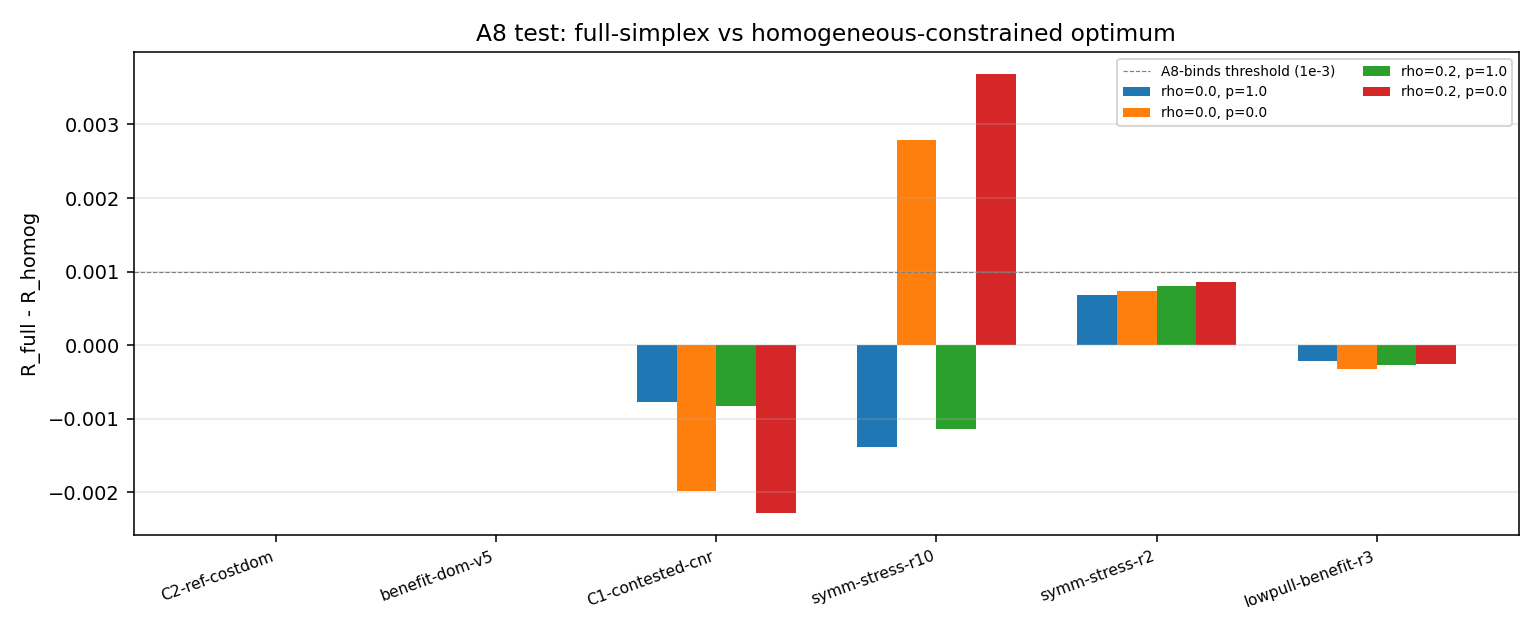
\includegraphics[width=0.92\textwidth]{figures/a8_simplex_dr.png}
  \caption{The rb-027 A8 N-dim sweep: $\Delta R = R_{\mathrm{full}}
    - R_{\mathrm{homog}}$ per panel across the six CR-036 decisive
    cells $\times$ $(\corr, p) \in \{0, 0.2\} \times \{0, 1\}$ ($24$
    panels). Bars above the dashed binding threshold $\Delta R =
    10^{-3}$ are A8-binding panels; the only two such panels are the
    symm-stress-r10 cell ($\valid = 0.25$, $\val = 1$, $\Rsens = 10$,
    variant~A) at $p = 0$ at both $\corr$ panels, with $\corr = 0.2$
    amplifying the binding by $32\%$ (Finding~2). Every $p = 1$ panel
    is below threshold (Finding~1, recovery). Source:
    \texttt{Rebuild/sims/A8--nd-uncued-sweep/}\allowbreak\texttt{output/figures/a8\_simplex\_dr.png}.}
  \label{fig:a8-simplex-dr}
\end{figure}

\paragraph{Finding 3: equal-split is a local maximum in every tested
panel — the Finding-2 binding is \emph{non-local}.}
At the homogeneous-$\alpha$ optimum of each of five Part~1 probe cells
(\texttt{v1-cost-dom}, \texttt{v1-reference}, \texttt{v1-symmetric},
\texttt{v1-benefit-dom}, \texttt{v1-lowV}, all at $\valid = 0.5$,
$\val = 1$, varying $\Rsens$), we compute the second derivative of
expected reward along the symmetry-preserving direction
$\mathbf{e}_{12} - 2\mathbf{e}_3$ on the uncued sub-simplex (a
redistribution that takes mass from one uncued slot and splits it
across the other two). Across the $5 \times 4 = 20$ panels of
$(\text{cell}, \corr, p)$, the curvature $R''(0)$ is negative in every
single panel — equal-split is a local maximum at the homogeneous
$\alpha^\star$ regardless of $(\corr, p)$. Combined with Finding~2,
this gives the binding a sharp \emph{non-local} character: the
homogeneous $\alpha_c \approx 0.05$ optimum of the symm-stress-r10
cell at $p = 0$ is \emph{locally stable} (the second-order
condition holds) but \emph{globally dominated} by the far-away
$\boldsymbol{\alpha}^\star = (0.5, 0, 0, 0.5)$ corner of the simplex.
The basin-hopping mechanism cannot be approximated by local gradient
information from the homogeneous policy; the only way to find the
binding is the global simplex search. Figure~\ref{fig:a8-curvature}
shows the curvature heatmap; every panel is negative (red below the
$R''(0) = 0$ line).

\begin{figure}[t]
  \centering
  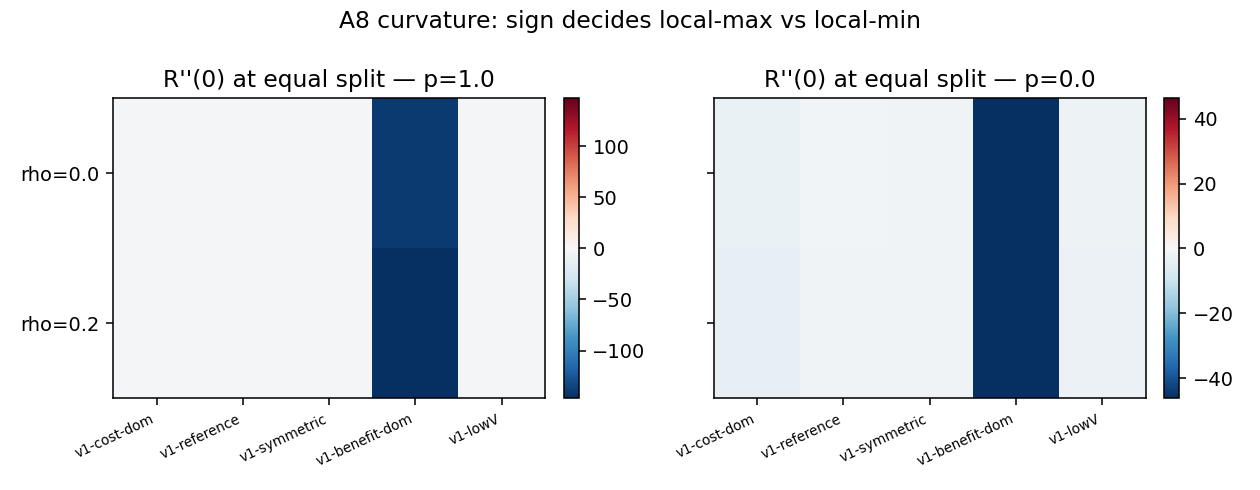
\includegraphics[width=0.85\textwidth]{figures/a8_curvature.png}
  \caption{The rb-027 Part~1 curvature panels: equal-split $R''(0)$
    along $\mathbf{e}_{12} - 2\mathbf{e}_3$ on the uncued sub-simplex
    at the homogeneous $\alpha^\star$, five probe cells $\times$ four
    $(\corr, p)$ panels (Finding~3). Every $R''(0)$ value is
    negative — equal-split is a local maximum in every tested panel.
    The Finding-2 A8 binding at the symm-stress-r10 cell ($p = 0$)
    is therefore non-local: the homogeneous $\alpha_c \approx 0.05$
    optimum is locally stable but globally dominated by the
    $(0.5, 0, 0, 0.5)$ corner. Source:
    \texttt{Rebuild/sims/A8--nd-uncued-sweep/}\allowbreak\texttt{output/figures/a8\_curvature.png}.}
  \label{fig:a8-curvature}
\end{figure}

\paragraph{Finding 4: A1 amplifies $|R''(0)|$ at $p = 1$ only
weakly — the A1$\times$A8 composition is more orthogonal than A1$\times$A2.}
At $p = 1$ (the inherited conservation rule), the ratio
$|R''(0)|_{\corr = 0.2} / |R''(0)|_{\corr = 0}$ across the five
Part~1 cells is reported in Table~\ref{tab:a8-rho-curv-ratio}. The
mean ratio is $1.048$ and the maximum is $1.135$ (\texttt{v1-reference});
the \texttt{v1-symmetric} cell actually \emph{suppresses} by $6\%$
(ratio $0.941$). Compare this to the rb-021 (A2) finding that the
analogous ratio for the equal-split criticality residual is
approximately $2\times$ (a $2.22\times$ ratio of the tangent gradient
$\|\mathbf{t}\|$ at $s = 0.3$, $5.81/2.61$, see
Section~\ref{sec:extensions-a2} Finding~1): the A1 channel composes
much more strongly with the A2 within-display heterogeneity lever
than with the A8 N-dim uncued lever. The rebuilt-model interpretation
is that A2 and A8 probe different aspects of the homogeneity
assumption: A2 breaks the per-location asymmetry $\Rsens_i = \Rsens$
exchange symmetry, which the joint no-FA integrand of the
$\corr$-channel inherits directly through the heterogeneous $\dprime_i$
vector; A8 breaks the per-location allocation $\alpha_i = (1\!-\!\alpha)/(\Nloc\!-\!1)$
exchange symmetry, which the joint no-FA integrand inherits only
through the second-order curvature of the equicorrelated
$\Nloc$-orthant integral on a homogeneous $\dprime$ — a higher-order
coupling that is small at $\corr = 0.2$.

\begin{table}[t]
  \centering
  \small
  \caption{Finding 4 (rb-027): $\corr$-amplification of the
    equal-split curvature $|R''(0)|$ at $p = 1$ across five Part~1
    cells ($\valid = 0.5$, $\val = 1$, varying $\Rsens$). Mean ratio
    $1.048$, maximum $1.135$, minimum $0.941$ (suppression). The A1
    amplification on the A8 equal-split criticality is small and
    non-uniform; cf.\ the rb-021 A2 finding of $\sim\!2\times$
    amplification on the analogous A2 criticality residual. Source:
    \texttt{Rebuild/sims/A8--nd-uncued-sweep/}\allowbreak\texttt{output/results.json}
    \texttt{summaries.rho\_amplification\_p1}; sha256~\texttt{beb2aa87\ldots}.}
  \label{tab:a8-rho-curv-ratio}
  \begin{tabular}{l r r r}
    \toprule
    cell tag & $|R''(0)|_{\corr = 0}$ & $|R''(0)|_{\corr = 0.2}$
      & ratio \\
    \midrule
    v1-cost-dom    & $2.261$  & $2.462$  & $1.089$ \\
    v1-reference   & $1.318$  & $1.496$  & $1.135$ \\
    v1-symmetric   & $1.750$  & $1.647$  & $0.941$ \\
    v1-benefit-dom & $141.0$  & $146.8$  & $1.041$ \\
    v1-lowV        & $2.269$  & $2.347$  & $1.035$ \\
    \bottomrule
  \end{tabular}
\end{table}

\paragraph{Finding 5: the anti-cued graded-suppression gradient
survives the A1 channel.}
The reviewer's CR-036 Part~2 establishes that the rebuilt model
under the inherited $\corr = 0$ reproduces the Wang \&
Theeuwes-style anti-cued suppression gradient: at a value-blind
($\val = 1$) cell with one slot \emph{less} likely to contain the
target than the others ($w_{\mathrm{anti}}$ swept from $0.20$ down to
$0$ while $\Nloc = 4$, $\valid = 0.40$ on the cued slot,
$w_{\mathrm{rest}} = (1\!-\!\valid\!-\!w_{\mathrm{anti}})/2$ on the
two intermediate slots, $\Rsens_c = 0.398$), the jointly-optimal
$(a_{\mathrm{cued}}, a_{\mathrm{anti}})$ shows $a_{\mathrm{anti}}^\star$
\emph{declining monotonically} as $w_{\mathrm{anti}}$ shrinks, and
$a_{\mathrm{anti}}^\star < a_{\mathrm{rest}}^\star$ strictly for every
$w_{\mathrm{anti}} > 0$ (a strictly graded statistical-learning-style
suppression). The rebuild's lift of this test to the A1 channel
$\corr \in \{0, 0.2\}$ recovers both qualitative features at both
$\corr$ panels: \emph{monotone} in $w_{\mathrm{anti}}$ and
\emph{strictly below} $a_{\mathrm{rest}}^\star$ are recorded as
\texttt{True} for every row of the Part~2 summary
(\texttt{summaries.anticued\_by\_rho}). $\corr = 0.2$ only weakly
perturbs the gradient: the value of $w_{\mathrm{anti}}$ at which
$a_{\mathrm{anti}}^\star$ collapses to zero is $w_{\mathrm{anti}} =
0.075$ at $\corr = 0$ ($a_{\mathrm{anti}}^\star$ drops from $0.02$ to
$0$) and $w_{\mathrm{anti}} = 0.050$ at $\corr = 0.2$
($a_{\mathrm{anti}}^\star$ drops from $0.02$ to $0$), shifted by one
grid step toward lower $w_{\mathrm{anti}}$. The behavioural reading
of CR-036 — that the rebuilt model offers a normative-optimal
mechanism for the graded suppression of statistical-distractor
locations that mirror-image the value-driven prioritisation observed
in valid-cue trials — therefore generalises across the A1 channel.
Figure~\ref{fig:a8-anticued-suppression} overlays the two $\corr$
panels. The strength ceiling here is the live A8 verdict's behavioural-
anchor sentence (``relaxing A8 lets the model reproduce the Wang \&
Theeuwes suppression gradient''): the rebuild does not claim the
suppression gradient is uniquely predicted by the rebuilt model, only
that the rebuilt model — with the A1 channel engaged — predicts it
under value-blind, statistically-shifted location-probability designs
\cite{wang_theeuwes2018_statistical_learning_distractor_suppression,failing_theeuwes2018_selection_history}.

\begin{figure}[t]
  \centering
  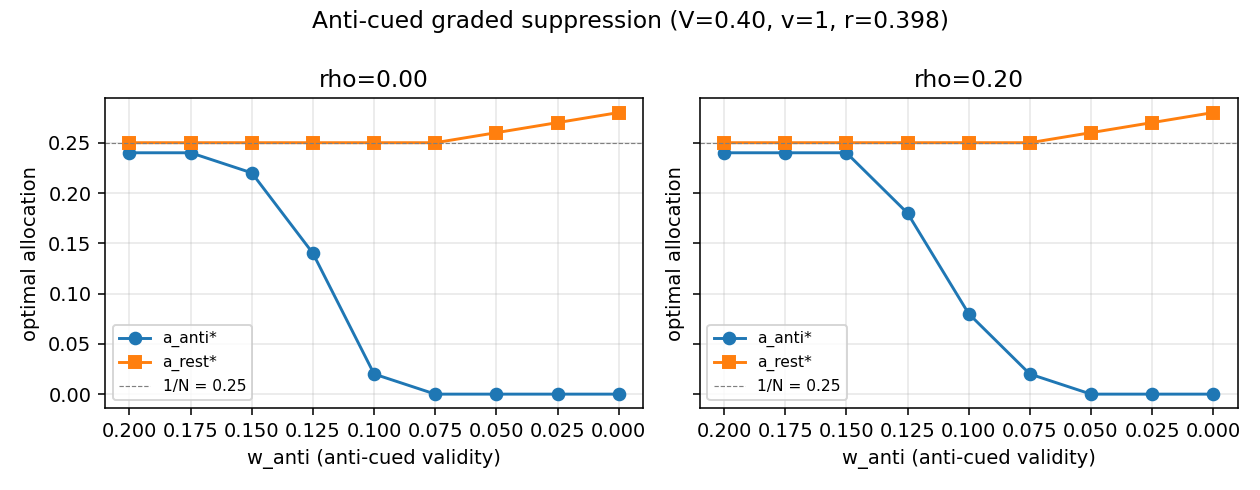
\includegraphics[width=0.85\textwidth]{figures/a8_anticued_suppression.png}
  \caption{The rb-027 Part~2 anti-cued graded-suppression gradient at
    $\corr \in \{0, 0.2\}$ (Finding~5). Jointly-optimal allocation
    $a_{\mathrm{anti}}^\star$ (solid) and $a_{\mathrm{rest}}^\star$
    (dashed) at the value-blind cell ($\Nloc = 4$, $\valid = 0.40$,
    $\val = 1$, $\Rsens_c = 0.398$, variant~A) as the anti-cued
    location's validity $w_{\mathrm{anti}}$ shrinks from $0.20$ down
    to $0$. $a_{\mathrm{anti}}^\star$ is monotone-decreasing and
    strictly below $a_{\mathrm{rest}}^\star$ at both $\corr$ panels;
    $\corr = 0.2$ shifts the collapse-to-zero of $a_{\mathrm{anti}}^\star$
    by one grid step toward lower $w_{\mathrm{anti}}$ (from
    $w_{\mathrm{anti}} = 0.075$ at $\corr = 0$ to $w_{\mathrm{anti}} =
    0.050$ at $\corr = 0.2$). The Wang--Theeuwes-style statistical-
    distractor suppression mechanism of CR-036 generalises across the
    A1 channel. Source:
    \texttt{Rebuild/sims/A8--nd-uncued-sweep/}\allowbreak\texttt{output/figures/a8\_anticued\_suppression.png}.}
  \label{fig:a8-anticued-suppression}
\end{figure}

\paragraph{Scope and what remains.}
This subsection licenses five claims at the rebuild-strength ceiling
of the live A8 verdict: (i) the inherited homogeneous-uncued allocation
lifts to the full $\Nloc$-simplex via \texttt{er\_full\_policy}, which
reproduces the inherited model under the canonical homogeneous
allocation to $\max|\Delta| \le 2.78\!\times\!10^{-10}$; (ii) under
the inherited $(\corr = 0, p = 1)$ pair, A8 is innocuous at every
CR-036 decisive cell — Finding~1 replicates the reviewer's headline
exactly; (iii) under multiplicative conservation $p = 0$, A8
\emph{binds} at the high-$\Rsens$ symmetric-stress benefit-dominant
corner ($\valid = 1/\Nloc$, $\val = 1$, $\Rsens = 10$, variant~A) by
$\Delta R = +2.79\!\times\!10^{-3}$ at $\corr = 0$ and
$+3.68\!\times\!10^{-3}$ at $\corr = 0.2$, a $32\%$ A1 amplification;
(iv) equal-split is a local maximum at the homogeneous $\alpha^\star$
in every $(\text{cell}, \corr, p)$ panel tested, so the Finding~2
binding is non-local; (v) the anti-cued graded-suppression gradient
of CR-036 Part~2 survives the A1 channel at $\corr \in \{0, 0.2\}$,
preserving the rebuilt model's Wang--Theeuwes-style behavioural-
anchor finding. The scope of these claims is explicitly bounded by
what the rb-027 sim ran and what it did \emph{not} run.
\emph{(i) Variant-B A8 binding.} The Finding~2 binding is reported
only at variant~A; the single variant-B cell in Part~1c
(\texttt{C1-contested-cnr}) shows $\Delta R < 0$ in all four
$(\corr, p)$ panels. A focused variant-B replication of the
symm-stress-r10 cell under $(\corr, p) \in \{0, 0.2\} \times \{0, 1\}$
is queued as RB-043, motivated by the rb-002 observation that
variant-B $\CF(\corr)$ is essentially flat at the headline cell
(Section~\ref{sec:model-upper-bound}). \emph{(ii) Finer $\Rsens$-grid.}
The Finding~2 binding is tested only at $\Rsens = 10$ on the
symm-stress cell; the $\Rsens$-axis location of the binding onset
(and termination, if any, on the lower end) is queued as RB-044
on a $6$-point $\Rsens$-grid around $\Rsens \in \{5, 10, 20\}$ at
fixed $\valid = 0.25$, $\val = 1$, variant~A. \emph{(iii) $\Nloc > 4$
generalisation.} All Part~1c panels are at $\Nloc = 4$; whether the
Finding~2 binding survives at larger $\Nloc$ (where the simplex
geometry has more degrees of freedom) is not in the rb-027 substrate.
\emph{(iv) Closed-form A8-binding boundary.} A closed-form predicate
for the A8-binding locus in $(\Rsens, p, \valid, \text{variant})$
space — a natural follow-up to Findings 1--2 — would consolidate the
empirical statement algebraically. A plausible substrate is a
Slepian-style monotonicity argument on the joint no-FA integrand
under simplex perturbation, but the Slepian inequality bounds
\emph{orthant probabilities}, not their gradients with respect to a
joint allocation; the derivation is not in the rebuild's voice and is
not queued. \emph{(v) Sim-boundary hardening.} The rb-027 sim
discovered a model-side numerical fragility: at small negative
$\alpha_i$ from float arithmetic in the simplex sweep,
\texttt{f\_transfer(alloc, $\ldots$, h=$\sqrt{\cdot}$)} returns NaN
which propagates through the criterion grid; the sim worked around
this at the boundary by clamping $\alpha_i \ge 0$ before passing to
\texttt{er\_full\_policy}. A model-side guard in
\texttt{d\_prime\_hetero} is queued as RB-045; this does not affect
any number reported here.

\paragraph{Reproducibility.}
The numerical content of this subsection is the
\texttt{Rebuild/sims/A8--nd-uncued-sweep/} simulation (rb-027,
deterministic sha256~\texttt{beb2aa879402e5c9f4c354a2c9f53a98c466d0989085dc8c78370be99dee290b},
$72.2$~s wall-clock on \texttt{python3.13} / \texttt{scipy 1.17.1} /
\texttt{numpy 2.4.4}; deterministic, re-run produces byte-identical
\texttt{results.json} and canonical \texttt{results.canonical.json}
verified empirically), backed by the
\texttt{Rebuild/model/\_\_init\_\_.py er\_full\_policy} driver wired
at rb-020. Four recovery contracts hold across this subsection,
none touched by the sim (the sim is a pure consumer of
\texttt{er\_full\_policy} and the four-test stack underneath it):
\textbf{Recovery~1 (A1 $\corr$-channel, rb-001).}
\texttt{test\_recovery.py} ($7/7$ PASS,
sha256~\texttt{d3c62215cedbe2f797c484a8d76e8bef1d5ac42cdb3092ff099a34aea1b6f18f}).
\textbf{Recovery~2 (A3 conservation family, rb-015).}
\texttt{test\_conservation\_family.py} ($14/14$ PASS,
sha256~\texttt{f4f57a89e5108db47447cbeaf2f15440f56cdfffb65f3d173dc4a0550121791e}).
\textbf{Recovery~3 (heterogeneous-$\Rsens$ d$'$-map, rb-019).}
\texttt{test\_heterogeneous\_r.py} ($5/5$ PASS,
sha256~\texttt{0486921f8a4e253a1682ee0731e52c7de800bf6c3dbb1b5e8ff3200602454c7e}).
\textbf{Recovery~4 (N-dim general policy, rb-020).}
\texttt{test\_general\_policy.py} ($7/7$ PASS,
sha256~\texttt{883ea15af9fd069e04c05ff156d65f33a7d25278891092539c6441d2248c3d39}).
Recovery~4 is the universal-statement guarantee for Finding~1: the
lifted \texttt{er\_full\_policy} reproduces the inherited
\texttt{optimal\_R} to $\max|\Delta| \le 2.78\!\times\!10^{-10}$
across $4{,}530$ cells at both $\corr \in \{0, 0.2\}$, so the
Finding~1 binding-fraction $0/6$ at $(\corr = 0, p = 1)$ is a
genuine reproduction of the reviewer's CR-036 Part~1c headline
rather than an artefact of a re-implementation.
